\documentclass[10pt,a4paper,twoside]{report}


%%%%%%%%%%%%%%%%%%%%%%%%%%%%%%%%%%%%%%%%%%%%%%%%%%%%%%%%%%%%%%%%%%%%%%%%%%
%%%%%%%%%%%%%%%%%%%%%%%%%%%%%%   PACKAGES   %%%%%%%%%%%%%%%%%%%%%%%%%%%%%%
%%%%%%%%%%%%%%%%%%%%%%%%%%%%%%%%%%%%%%%%%%%%%%%%%%%%%%%%%%%%%%%%%%%%%%%%%%
\usepackage[french]{babel} % Babel est un package qui permet d'obtenir des documents en plusieurs langues, en respectant les typographies nationales, en affichant automatiquement les titres (comme « table des matières », « index », etc) dans la langue choisie, etc.  On peut aussi utiliser babel pour écrire un document en plusieurs langues. Pour cela, il faut lui donner en option la liste de toutes les langues qui seront utilisées en plaçant en dernier la langue principale du document. Pour alterner entre les langues, on utilise la commande : \selectlanguage{nom-de-la-langue}
%\usepackage{standalone}
\usepackage{graphicx}
\usepackage{numprint} % de regrouper les milliers avec la commande \nombre{}
%\usepackage[utf8]{inputenc} % L'inclusion de ce package permet d'utiliser des sources LaTeX contenant des caractères accentués. L'option [latin1]  précise que l'encodage des fichiers est iso-latin1 ou iso iso-8859-1. En effet, sans cette extension, il est nécessaire d'utiliser une syntaxe particulière pour l'affichage des accents. --> Pas nécéssaire en UTF-8
\usepackage{comicneue} % Pour avoir des polices comicneuesur tout le document. Beaucoup plus jolie et agréable à lire
\usepackage[T1]{fontenc} % Permet de spécifier à LaTeX l'utilisation du codage de caractères T1, nouvelle norme LaTeX non utilisée par défaut pour des raisons de compatibilité avec les anciens documents LaTeX.
%\usepackage[francais]{layout} % Est une sorte de bibiothèque de fonction contenant la fonction utile "\layout" qui dessine la structure physique du documents et indique leurs dimensions.
\usepackage{amssymb} % Permet d'utiliser différents symbôles mathématiques.
\usepackage[fleqn]{amsmath} % Permet d'utiliser différents environnements propices aux maths. L'option "fleqn" permet de ne pas centrer l'environnement "align" en conjnction avec la commande \setlength{\mathindent{0pt}}
\usepackage{ulem} % Ce package permet de faire différents types de sous ou sur-lignements. (Comme le double souslignements par exemple).
\usepackage{fancyhdr}  %package pour en-tetes et pied de pages
\usepackage{sectsty} % Permet de faire des modifications de police dans diverses sections des "headings" (cf. modif presentation de la page)
%\usepackage{titlesec}
\usepackage[svgnames,table]{xcolor}   % Permet de définir des nouvelles couleurs (peut-être aussi d'utiliser les couleurs en général)
\usepackage{color}   % Permet de définir des nouvelles couleurs (peut-être aussi d'utiliser les couleurs en général)
\usepackage{lastpage} % Permet à Latex d'identifier la dernière page du document avec la commande "\"
\usepackage[inline]{enumitem} % Permet de préciser des options lors de la déclaration de l’environnement d’une liste à puces
% \usepackage{enumerate} % Permet de faire des liste numérotées avec des i) ; ii) etc... 
\usepackage{shadowtext} % Permet de faire du text avec des ombres
%\usepackage{showframe} % Permet de montrer les marges du document
\usepackage{blindtext} % permet de générer un text avec la commande "\blindtext" afin de tester des macros et autres environnements
\usepackage{tikz} % Permet de faire des dessins avec les commandes Tikz
%\usepackage{auto-pst-pdf}

%\usepackage{pstricks,pst-plot,pstricks-add}

\usepackage{pst-func}
%\usepackage{fourier} % Change la police (assez joli) et permet de faire le sympbole attention: \danger
\usepackage{bold-extra}
%\usepackage{fontspec} % Package pour le polices de caractères
\usetikzlibrary{shapes} %Shape library, used to define shapes other than rectangle, circle and co-ordinate. The following additional types are available: geometric shapes, either named shapes (star, diamond, etc.) or polygons of specified side numbers; symbol shapes, e.g. "forbidden sign" as used in No Smoking signs; "multipart" shapes, with "multiple (text) parts"; and finally, "misc" shapes which "do not fit in the previous categories", such as strikethrough crosses.
\usetikzlibrary{shadows.blur}
\usepackage{bm} % permet de faire des symbole mathématique en gras avec \boldsymbol{}
\usepackage[thicklines]{cancel}
%\usepackage{phantom}
\usepackage{calc}
\usepackage{multicol}
\usepackage{stackengine}
\usepackage{nicefrac} % permet de faire de fraction "oblique"
\usepackage{tkz-tab} % pour les tableaux de variations
\usepackage{wrapfig} % permet de faire "couler" du texte autour d'une figure
\usepackage{setspace} % pour les commandes sur les interlignes
\usepackage[charter]{mathdesign} % Pour avoir des polices en mathdesign
\usepackage{hyperref} % Pour pouvoir inclure des informations au fichier pdf -> /!\ elle définit la command "\C", d'où une REdéfinition les "commandes" de "\C".
\usepackage{paracol}
%\usepackage[bottom]{footmisc} % option pour mettre les notes colées au pied de la page et nom au text du corps.
\usepackage{amsthm}
\usepackage{tcolorbox}
%\usepackage{siunitx} % Pour les unités
%\usepackage{yhmath} % Pour faire des "arcs" sur les lettres pour les arcs de cercles : "\wideparen{AB}"
\usepackage{tasks} % Pour faire des listes en multicolonnes "horizontalement"
\usepackage{titlesec}
\usepackage{mathtools} % Notamment pour utiliser pmatrix* dont * l'étoile permet de d'aligner les nombres indépendemment des signes
\usepackage{thmtools}
\usepackage{polynom} % Pour effectuer les divisions euclidiennes
\usepackage{lipsum}
\usepackage{textcomp} %Pour faire des fractions avec les commandes \textonehalf, \textonequarter, \textthreequarters
\usepackage{array}
\usepackage{afterpage} % pour insérer des pages blanches (a étudier...)
\usepackage{icomma}


%\usepackage{shortlst}
%\usepackage{paralist}


%%%%%%%%%%%%%%%%%%%%%%%%%%%%%%%%%%%%%%%%%%%%%%%%%%%%%%%%%%%%%%%%%%%%%%%%%%
%%%%%%%%%%%%%%%%%%%%%%%%%%%   ENVIRONNEMENTS   %%%%%%%%%%%%%%%%%%%%%%%%%%%
%%%%%%%%%%%%%%%%%%%%%%%%%%%%%%%%%%%%%%%%%%%%%%%%%%%%%%%%%%%%%%%%%%%%%%%%%%
% La différence entre \arabic{compteur} et \thecompteur se remarque si compteur est « lié » à un autre compteur. Un compteur est lié à un autre si ce premier est réinitialisé lorsque le second est incrémenté. Par exemple dans la classe book, les figures sont numérotées en commençant par le numéro du chapitre. Ainsi, la deuxième figure du chapitre 3 est numérotée « 3.2 », et la valeur de \arabic{figure} est alors « 2 », tandis que celle de \thefigure est « 3.2 ».

%La différence étant que refstepcounter donne à la commande \ref{label} la même que \thecompteur (au lieu de \arabic{compteur}, vous suivez ?).

% informations provenant de : http://blog.dorian-depriester.fr/latex/les-compteurs-sous-latex#Personnaliser_lrsquoaffichage_du_compteur

\tcbuselibrary{theorems, skins, breakable} % Pour utiliser certaines commandes du package "tcolorbox"

\usetikzlibrary{shadows}




%%%%%%%%%%%%%%%%%%%%%%%%%%%%%%%%%%%%%%%%%%%%%%%%%%%%%%%%%%%%%%%%%%%
%%%%%%%%%%%%%% Personalisations de tcolorbox
%%%%%%%%%%%%%%%%%%%%%%%%%%%%%%%%%%%%%%%%%%%%%%%%%%%%%%%%%%%%%%%%%%%
\tcbset{
	semiboxedshadow/.style 2 args={
			enhanced, colback=gray!20, colframe=gray!10,rounded corners, arc=3mm, left=4mm,top=4mm, bottom=3mm,%boxrule=0pt,
			%borderline west={#1}{0pt}{#2},left={#1*14/10+7pt},top=1ex, bottom=1ex,
			%borderline south={#1}{0pt}{#2},left={#1*14/10+7pt},top=1ex, bottom=1ex,
			fuzzy shadow={1mm}{-1mm}{0mm}{0.3mm}{fill=black,opacity=0.25},			
			%drop fuzzy shadow,
			after skip=5mm
			},
	leftlined/.style 2 args={
			blanker, breakable,
			borderline west={#1}{0pt}{#2},left={#1*14/10+7pt},top=1ex, bottom=1ex,
			},
    exstyle/.style={enhanced, colback=Indigo!5, colframe=Indigo, 
           fonttitle=\bfseries, 
           colbacktitle=Indigo, coltitle=white,  
           top=2mm,
           boxed title style={},
           attach boxed title to top left={yshift=-\tcboxedtitleheight/2,xshift=4mm}%
           },
    teostyle/.style={enhanced, colback=white, colframe=White, 
           fonttitle=\bfseries, sharp corners, boxrule=0pt,
           colbacktitle=Red!100, coltitle=white,
           drop fuzzy shadow,  
           top=2mm,
           boxed title style={sharp corners},
           attach boxed title to top left={}%
           },
	indented/.style={
			blanker, breakable,left=#1, colback=white, %colframe=white,
			%borderline west={#1}{0cm}{#2},left={#1*30/10+7pt},top=1ex, bottom=1ex,
			}, 
}


%\newtcbtheorem[number within=section]{miTeorema}{Teorema}{teostyle}{teo}

% CI DESSOUS UN EXEMPLE D'UTILISATION DU STYLE "THEOSTYLE" CI-DESSUS :
%\begin{miTeorema}{Un teorema}{label}
%Sean $a, b\in \mathbb{Z}$ con $b\neq 0$ . Sea $q\in \mathbb{Z}$ \dots
%\end{miTeorema}



%%%%%%%%%%%%%%%%%%%%%%%%%%%%%%%%%%%%%%%%%%%%%%%%%%%%%%%%%%%%%%%%%%%
%%%%%%%%%%%%%% DEFINITION 
%%%%%%%%%%%%%%%%%%%%%%%%%%%%%%%%%%%%%%%%%%%%%%%%%%%%%%%%%%%%%%%%%%%
\newtheoremstyle{definition}% name
{3pt}% Space above  % -> NE MARCHE PAS - CERTAINEMENT A CAUSE DE TCB QUI DOIT "OVERRULER" LES DIMENSIONS
{3pt}% Space below  % -> NE MARCHE PAS - CERTAINEMENT A CAUSE DE TCB QUI DOIT "OVERRULER" LES DIMENSIONS
{}% Body font \itshape
{}% Indent amount
{\bfseries\large}% Theorem head font
{\vspace{1mm}\newline}% Punctuation after theorem head
{1mm}%{0pt\Needspace{3\baselineskip}}% Space after theorem head % -> NE MARCHE PAS - CERTAINEMENT A CAUSE DE TCB QUI DOIT "OVERRULER" LES DIMENSIONS
{}% Theorem head spec (can be left empty, meaning ‘normal’ )
%
%\newtheoremstyle{definitions}% name
%{3pt}% Space above  % -> NE MARCHE PAS - CERTAINEMENT A CAUSE DE TCB QUI DOIT "OVERRULER" LES DIMENSIONS
%{3pt}% Space below  % -> NE MARCHE PAS - CERTAINEMENT A CAUSE DE TCB QUI DOIT "OVERRULER" LES DIMENSIONS
%{}% Body font \itshape
%{}% Indent amount
%{\bfseries}% Theorem head font
%{\vspace{1mm}\newline}% Punctuation after theorem head
%{1mm}%{0pt\Needspace{3\baselineskip}}% Space after theorem head % -> NE MARCHE PAS - CERTAINEMENT A CAUSE DE TCB QUI DOIT "OVERRULER" LES DIMENSIONS
%{}% Theorem head spec (can be left empty, meaning ‘normal’ )

%\tcolorboxenvironment{definition}{exstyle}
%\tcolorboxenvironment{definition}{teostyle}


\tcolorboxenvironment{definition}{semiboxedshadow}
\tcolorboxenvironment{definitions}{semiboxedshadow}
\tcolorboxenvironment{definitiond}{semiboxedshadow}
\tcolorboxenvironment{definitionsd}{semiboxedshadow}



\theoremstyle{definition}
\newtheorem{definition}{Définition}[chapter]
\newtheorem{definitiond}[definition]{Définition*}
\newtheorem{definitions}[definition]{Définitions}
\newtheorem{definitionsd}[definition]{Définitions*}


%\newenvironment{importantbarre}





%%%%%%%%%%%%%%%%%%%%%%%%%%%%%%%%%%%%%%%%%%%%%%%%%%%%%%%%%%%%%%%%%%%
%%%%%%%%%%%%%% THEOREME - PROPOSITION - LEMME %%%%%
%%%%%%%%%%%%%%%%%%%%%%%%%%%%%%%%%%%%%%%%%%%%%%%%%%%%%%%%%%%%%%%%%%%
\newtheoremstyle{theoreme}% name
	{3pt}% Space above
	{3pt}% Space below
	{\itshape}% Body font
	{}% Indent amount
	{\bfseries\large}% Theorem head font
	{\vspace{1mm}\newline}% Punctuation after theorem head
	{1cm}%{0pt\Needspace{3\baselineskip}}% Space after theorem head
	{}% Theorem head spec (can be left empty, meaning ‘normal’ )


\newtheoremstyle{theoremeavance}% name
    {3pt}%   Space above
    {3pt}%   Space below
    {\itshape}%  Body font
    {}%          Indent amount
    {\bfseries\large}% Theorem head font
    {\vspace{1mm}\newline}%          Punctuation after theorem head -- blank
    {1cm}%     Space after theorem head (0.5em is the default)
    {{\thmname{#1}\thmnumber{ #2$^{\bm*}\!$}\thmnote{\ \textmd{(#3)}}}}% Theorem head spec 

\theoremstyle{theoreme}
\newtheorem{theoreme}{Théorème}[chapter]
\newtheorem{proposition}[theoreme]{Proposition}
\newtheorem{lemme}[theoreme]{Lemme}
\newtheorem{corolaire}[theoreme]{Corolaire}

\theoremstyle{theoremeavance}
\newtheorem{theoremed}[theoreme]{Théorème}
\newtheorem{propositiond}[theoreme]{Proposition}
\newtheorem{lemmed}[theoreme]{Lemme}
\newtheorem{corolaired}[theoreme]{Corolaire}

\tcolorboxenvironment{theoreme}{leftlined={5pt}{red!40!darkgray}}
\tcolorboxenvironment{theoremed}{leftlined={5pt}{red!40!darkgray}}
\tcolorboxenvironment{proposition}{leftlined={5pt}{red!40!darkgray}}
\tcolorboxenvironment{propositiond}{leftlined={5pt}{red!40!darkgray}}
\tcolorboxenvironment{lemme}{leftlined={5pt}{red!40!darkgray}}
\tcolorboxenvironment{lemmed}{leftlined={5pt}{red!40!darkgray}}
\tcolorboxenvironment{corolaire}{leftlined={5pt}{red!40!darkgray}}
\tcolorboxenvironment{corolaired}{leftlined={5pt}{red!40!darkgray}}
%\newtcbtheorem[number within=chapter]{proposition}{Proposition}
%\declaretheorem[style=proposition]{named}

%\theoremstyle{theoremeavance}
%\newtheorem{theoremeavance}[theoreme]{Théorème}
%\newtheorem{propositionavancee}[theoreme]{Proposition}


\newtheoremstyle{demonstration}% name
{3pt}% Space above
{3pt}% Space below
{}% Body font
{-10pt}% Indent amount
{\itshape}% Theorem head font
{\vspace{1mm}\newline}% Punctuation after theorem head
{1cm}%{0pt\Needspace{3\baselineskip}}% Space after theorem head
{}% Theorem head spec (can be left empty, meaning ‘normal’ )


\theoremstyle{demonstration}
\newtheorem*{demonstration}{Démonstration :}
\newtheorem*{demonstrationd}{Démonstration$^{*}\!$ :}

\tcolorboxenvironment{demonstration}{indented={10pt}}
\tcolorboxenvironment{demonstrationd}{indented={10pt}}









%%%%%%%%%%%%%%%%%%%%%%%%%%%%%%%%%%%%%%%%%%%%%%%%%%%%%%%%%%%%%%%%%%%
%%%%%%%%%%%%%% CONFLIT AVEC L'ENVIRONNEMENT DES ALGORItHMES
%%%%%%%%%%%%%%%%%%%%%%%%%%%%%%%%%%%%%%%%%%%%%%%%%%%%%%%%%%%%%%%%%%%
%%-----------------------
%%---- Démonstration ----
%%-----------------------
%\newtheoremstyle{demonstration}% name
%{3pt}% Space above  % -> NE MARCHE PAS - CERTAINEMENT A CAUSE DE TCB QUI DOIT "OVERRULER" LES DIMENSIONS
%{3pt}% Space below  % -> NE MARCHE PAS - CERTAINEMENT A CAUSE DE TCB QUI DOIT "OVERRULER" LES DIMENSIONS
%{}% Body font \itshape
%{-10mm}% Indent amount
%{\itshape}% Theorem head font
%{\vspace{2.5mm}\newline}% Punctuation after theorem head
%{1mm}%{0pt\Needspace{3\baselineskip}}% Space after theorem head % -> NE MARCHE PAS - CERTAINEMENT A CAUSE DE TCB QUI DOIT "OVERRULER" LES DIMENSIONS
%{}% Theorem head spec (can be left empty, meaning ‘normal’ )
%
%\theoremstyle{demonstration}
%\tcolorboxenvironment{demonstration}{indented={8mm}}
%\newtheorem*{demonstration}{Démonstration :}







%%%%%%%%%%%%%%%%%%%%%%%%%%%%%%%%%%%%%%%%%%%%%%%%%%%%%%%%%%%%%%%%%%%
%%%%%%%%%%%%%% EXERCICES 
%%%%%%%%%%%%%%%%%%%%%%%%%%%%%%%%%%%%%%%%%%%%%%%%%%%%%%%%%%%%%%%%%%%
\tikzset{
     shadowed/.style={preaction={transform canvas={shift={(-1pt,-1pt)}},draw=gray,very thick}},
  }
\newcounter{exercice}
% couleurchapitre est définit dans le préambule du document maître
%\newtcolorbox[use counter=exercice]{exstheorie}{
\newtcolorbox{boxexstheorie}{
empty,
coltext=gray!10!black,
title={Exercices},
attach boxed title to top left,
boxed title style={
	toprule=2pt,top=2pt,left=0cm,overlay={
		\path[left color=white, right color=couleurchapitre,rounded corners=5pt]([yshift=0pt]frame.north east)+(0cm,-23pt) rectangle +(-4.5cm,0pt);}
},
coltitle=white,fonttitle=\Large\bfseries\itshape,
before=\par\medskip\noindent,parbox=false,boxsep=0pt,left=0cm,right=3mm,top=2mm,bottom=5mm,
breakable, pad at break*=0mm,vfill before first,
%overlay unbroken={\draw[couleurchapitre,line width=1pt,shadowed]
%([xshift=0mm,yshift=0pt]title.south east)--([xshift=0mm]title.south-|frame.east); },
%([xshift=-15mm,yshift=-1pt]title.south-|frame.west)--([xshift=-15mm]frame.south west); },%--(frame.south),
%overlay first={\draw[couleurchapitre,line width=1pt,shadowed]
%([xshift=-15mm,yshift=-1pt]title.south-|frame.west)--([xshift=-15mm]frame.south west); },
%overlay middle={\draw[couleurchapitre,line width=1pt,shadowed]
%([xshift=-15pt]frame.north west)--([xshift=-15pt]frame.south west); },
%overlay last={\draw[couleurchapitre,line width=1pt,shadowed]
%([xshift=-25pt]frame.north west)--([xshift=-25pt]frame.south west)--(frame.south);},%
}

\newenvironment{exstheorie}
	{
         \begin{boxexstheorie}%
            \raggedcolumns
			\columnseprule=1.pt
			\columnsep=40pt
			\renewcommand{\columnseprulecolor}{\color{gray}}
			\vspace*{-3mm}
			\begin{multicols*}{2}
				\flushcolumns
				\columnseprule=0pt
    }
	{                		
			\end{multicols*}
		\end{boxexstheorie}%
	}
	
\newenvironment{exstheoriesansligne}
	{
         \begin{boxexstheorie}%
            \raggedcolumns
			\columnsep=40pt
			\begin{multicols*}{2}
				\flushcolumns
				\columnseprule=0pt
    }
	{                		
			\end{multicols*}
		\end{boxexstheorie}%
	}

%\newenvironment{exstheorie}
%	{
%		\begin{multicols*}{2}
%         \begin{boxexstheorie}%
%            \raggedcolumns
%			\columnseprule=1.pt
%			\columnsep=40pt
%			\renewcommand{\columnseprulecolor}{\color{gray}}
%				\flushcolumns
%				\columnseprule=0pt
%    }
%	{
%		\end{boxexstheorie}%                		
%		\end{multicols*}
%	}



%\newtcolorbox{boxexstheorieligne}{
%empty,
%coltext=gray!10!black,
%title={Exercices},
%attach boxed title to top left,
%boxed title style={
%	toprule=2pt,top=2pt,left=-0.3cm,overlay={
%		\path[left color=white, right color=couleurchapitre,rounded corners=5pt]([yshift=0pt]frame.north east)+(0.5cm,-23pt) rectangle +(-4.5cm,0pt);}
%},
%coltitle=white,fonttitle=\Large\bfseries\itshape,
%before=\par\medskip\noindent,parbox=false,boxsep=0pt,left=-1.3cm,right=3mm,top=2mm,bottom=5mm,
%breakable, pad at break*=0mm,vfill before first,
%overlay unbroken={\draw[couleurchapitre,line width=1pt,shadowed]
%([xshift=0mm,yshift=0pt]title.south east)--([xshift=0mm]title.south-|frame.east); ,
%([xshift=-15mm,yshift=-1pt]title.south-|frame.west)--([xshift=-15mm]frame.south west); },%--(frame.south),
%overlay first={\draw[couleurchapitre,line width=1pt,shadowed]
%([xshift=-15mm,yshift=-1pt]title.south-|frame.west)--([xshift=-15mm]frame.south west); },
%overlay middle={\draw[couleurchapitre,line width=1pt,shadowed]
%([xshift=-15pt]frame.north west)--([xshift=-15pt]frame.south west); },
%overlay last={\draw[couleurchapitre,line width=1pt,shadowed]
%([xshift=-25pt]frame.north west)--([xshift=-25pt]frame.south west)--(frame.south);},%
%}



%\newtcolorbox{boxexstheorieligne}{
%empty,
%coltext=gray!10!black,
%title={Exercices},
%attach boxed title to top left,
%boxed title style={
%	toprule=2pt,top=2pt,left=-1.3cm,overlay={
%		\path[left color=white, right color=couleurchapitre,rounded corners=5pt]([yshift=0pt]frame.north east)+(0.5cm,-23pt) rectangle +(-4.5cm,0pt);}
%},
%coltitle=white,fonttitle=\Large\bfseries\itshape,
%before=\par\medskip\noindent,parbox=false,boxsep=0pt,left=-1.3cm,right=3mm,top=2mm,bottom=5mm,
%breakable, pad at break*=0mm,vfill before first,
%overlay unbroken={\draw[couleurchapitre,line width=1pt,shadowed]
%([xshift=0mm,yshift=0pt]title.south east)--([xshift=0mm]title.south-|frame.east); ,
%([xshift=-15mm,yshift=-1pt]title.south-|frame.west)--([xshift=-15mm]frame.south west); },%--(frame.south),
%overlay first={\draw[couleurchapitre,line width=1pt,shadowed]
%([xshift=-15mm,yshift=-1pt]title.south-|frame.west)--([xshift=-15mm]frame.south west); },
%overlay middle={\draw[couleurchapitre,line width=1pt,shadowed]
%([xshift=-15pt]frame.north west)--([xshift=-15pt]frame.south west); },
%overlay last={\draw[couleurchapitre,line width=1pt,shadowed]
%([xshift=-25pt]frame.north west)--([xshift=-25pt]frame.south west)--(frame.south);},%
%}



%%%\newcounter{exercices}
%\newtcolorbox[use counter=exercice]{boxexstheorieligne}{%
%empty,
%title={Example \thetcbcounter},
%attach boxed title to top left,
%boxed title style={
%	toprule=2pt,top=2pt,left=-0.6cm,overlay={
%		\path[left color=white,right color=couleurchapitre,rounded corners=5pt]([yshift=0pt]frame.north east)+(0cm,-23pt) rectangle +(-5cm,0pt);}
%},
%coltitle=couleurchapitre,fonttitle=\Large\bfseries,
%before=\par\medskip\noindent,parbox=false,boxsep=0pt,left=0pt,right=3mm,top=4pt,
%breakable,pad at break*=1mm,vfill before first,
%overlay unbroken={\draw[couleurchapitre,line width=1pt]
%([yshift=-1pt]title.north east)--([xshift=-0.5pt,yshift=-1pt]title.north-|frame.east)--([xshift=-0.5pt]frame.south east)--(frame.south west); },
%overlay first={\draw[couleurchapitre,line width=1pt,shadowed]
%([yshift=-1pt]title.south-|frame.west)--([xshift=-0.5pt,yshift=-1pt]title.north-|frame.east)--([xshift=-0.5pt]frame.south east); },
%overlay middle={\draw[couleurchapitre,line width=1pt]
%([xshift=-0.5pt]frame.north east)--([xshift=-0.5pt]frame.south east); },
%overlay last={\draw[couleurchapitre,line width=1pt]
%([xshift=-10pt]frame.north west)--([xshift=-10pt]frame.south west)--(frame.south);},%
%}




%%\newcounter{exercices}
%\tikzset{
%     shadowed/.style={preaction={transform canvas={shift={(-1pt,-1pt)}},draw=gray,very thick}},
%  }
\newtcolorbox[use counter=exercice]{boxexstheorieligne}{%
empty,
title={Exercices},
attach boxed title to top left,
boxed title style={
	toprule=2pt,top=2pt,left=-0.1cm,overlay={
		\path[left color=white, right color=couleurchapitre,rounded corners=5pt]([yshift=0pt]frame.north east)+(0cm,-23pt) rectangle +(-5cm,0pt);}
},
coltitle=white,fonttitle=\Large\bfseries\itshape,
before=\par\medskip\noindent,parbox=false,boxsep=0pt,left=0pt,right=3mm,top=12pt,
breakable,pad at break*=1mm,vfill before first,
overlay unbroken={\draw[couleurchapitre,line width=2pt,shadowed]
([xshift=-15pt,yshift=-1pt]title.south-|frame.west)--([xshift=-15pt,yshift=-5pt]frame.south west)--([xshift=-0.5pt,yshift=-5pt]frame.south);},%--(frame.south west); },
%-------------------------------------------------------------------------
overlay first={\draw[couleurchapitre,line width=2pt,shadowed]
([xshift=-15pt,yshift=-1pt]title.south-|frame.west)--([xshift=-15pt,yshift=-10pt]frame.south west);},%--([xshift=-0.5pt,yshift=-10pt]frame.south);}--(frame.south west); },
%-------------------------------------------------------------------------
overlay middle={\draw[couleurchapitre,line width=2pt,shadowed]
([xshift=-15pt]frame.north west)--([xshift=-15pt]frame.south west); },
%-------------------------------------------------------------------------
overlay last={\draw[couleurchapitre,line width=2pt,shadowed]
([xshift=-15pt]frame.north west)--([xshift=-15pt]frame.south west)--(frame.south);},%
}



%\newenvironment{exstheorieligne}
%	{
%         \begin{boxexstheorieligne}%
%
%		\end{boxexstheorieligne}%
%	}

%%% LA VERSION CI-DESSOUS (exstheorieligne) EST L'ORIGINALE QUI N'EST PLUS UTILISEE. PAR AILLEURS, IL Y A UN PROBLEME LORS DU CHAGMENT DE PAGE CAR LES TRAITS DECORATIFS NE SE FONT PAS SUR LA 2EME PAGE.
%\newcounter{exercices}
\colorlet{colexam}{gray!75!black}
\newtcolorbox[use counter=exercice]{exstheorieligne}{%
empty,title={Exercices},attach boxed title to top left,
boxed title style={empty,size=minimal,toprule=2pt,top=6pt,overlay={\draw[colexam,line width=2.5pt]([yshift=-1pt]frame.north west)--([yshift=-1pt]frame.north east);}},
coltitle=black,fonttitle=\Large\bfseries\itshape,
before=\par\medskip\noindent,parbox=false,boxsep=0pt,left=10pt,right=3mm,top=10pt,
breakable,pad at break*=0mm,vfill before first,
overlay unbroken={\draw[colexam,line width=1pt]
([yshift=-1pt]title.north east)--([xshift=-0.5pt,yshift=-1pt]title.north-|frame.east)
--([xshift=-0.5pt]frame.south east)--(frame.south west); },
overlay first={\draw[colexam,line width=1pt]
([yshift=-1pt]title.north east)--([xshift=-0.5pt,yshift=-1pt]title.north-|frame.east)
--([xshift=-0.5pt]frame.south east); }%,
overlay middle={\draw[colexam,line width=1pt] ([xshift=-0.5pt]frame.north east)
--([xshift=-0.5pt]frame.south east); }%,
overlay last={\draw[colexam,line width=1pt] ([xshift=-0.5pt]frame.north east)
--([xshift=-0.5pt]frame.south east)--(frame.south west);}%,%
}

%%%%%%%%%%%%%%%%%%%%%%%%%%%%%%%%
%D'autres possibilités pour les exercices. A travailler.
%%%%%%%%%%%%%%%%%%%%%%%%%%%%%%%%
%
%\begin{tcolorbox}[enhanced,colframe=gray!75!white,interior style={left color=gray!30,right color=white},leftrule=3mm,title=Exercices]
%This is the upper part.
%
%This is the lower part.
%\end{tcolorbox}
%
%%%%%%%%%%%%%%%%%%%%%%%%%%%%%%%%
%
%\begin{tcolorbox}[enhanced,sharp corners=south,
%colframe=red!75!black,interior style={top color=white,bottom color=red!50}]
%This is an example for 'spread downwards'.
%\end{tcolorbox}
%
%%%%%%%%%%%%%%%%%%%%%%%%%%%%%%%%
%
%\newtheoremstyle{exercice}% name
%{3pt}% Space above  % -> NE MARCHE PAS - CERTAINEMENT A CAUSE DE TCB QUI DOIT "OVERRULER" LES DIMENSIONS
%{3pt}% Space below  % -> NE MARCHE PAS - CERTAINEMENT A CAUSE DE TCB QUI DOIT "OVERRULER" LES DIMENSIONS
%{\itshape}% Body font \itshape
%{-2mm}% Indent amount
%{\bfseries\itshape}% Theorem head font
%{\newline}% Punctuation after theorem head
%{1mm}%{0pt\Needspace{3\baselineskip}}% Space after theorem head % -> NE MARCHE PAS - CERTAINEMENT A CAUSE DE TCB QUI DOIT "OVERRULER" LES DIMENSIONS
%{}% Theorem head spec (can be left empty, meaning ‘normal’ )
%
%\theoremstyle{exercice}
%\tcolorboxenvironment{exercice}{exstyle}
%\newtheorem*{exercice}{Exercice :}
%
%
%%-------------------
%%---- ExerciceS ----
%%-------------------
%\newtheoremstyle{exercices}% name
%{3pt}% Space above  % -> NE MARCHE PAS - CERTAINEMENT A CAUSE DE TCB QUI DOIT "OVERRULER" LES DIMENSIONS
%{3pt}% Space below  % -> NE MARCHE PAS - CERTAINEMENT A CAUSE DE TCB QUI DOIT "OVERRULER" LES DIMENSIONS
%{\itshape}% Body font \itshape
%{-2mm}% Indent amount
%{\bfseries\itshape}% Theorem head font
%{\newline}% Punctuation after theorem head
%{1mm}%{0pt\Needspace{3\baselineskip}}% Space after theorem head % -> NE MARCHE PAS - CERTAINEMENT A CAUSE DE TCB QUI DOIT "OVERRULER" LES DIMENSIONS
%{}% Theorem head spec (can be left empty, meaning ‘normal’ )
%
%\theoremstyle{exercices}
%\tcolorboxenvironment{exercices}{indented={1mm}}
%\newtheorem*{exercices}{Exercices :}








%%%%%%%%%%%%%%%%%%%%%%
%---- Indications ----
%%%%%%%%%%%%%%%%%%%%%%
\newcommand{\indication}[2]{\footnotesize\textit{(\textbf{Indication :} \begin{minipage}[t]{#1\linewidth} #2)\end{minipage}}\normalsize}

\newcommand{\indicationsansparentheses}[2]{\footnotesize\it\begin{minipage}[t]{#1\textwidth}
 \textbf{Indication : } #2
\end{minipage}\normalsize}








%%%%%%%%%%%%%%%%%%%%%%%%%%%%%%%%%%%%%%%%%%%%%%%%%%%%%%%%%%%%%%%%%%%%%%%%%%%%%%%%%%%%%%%%%%%%%%
%%%%%%%%%%%%%%%%%%  CODE POUR ENTRER DIRECTEMENT DES FICHIERS PYTHON  %%%%%%%%%%%%%%%%%%%%%%%%
%%%%%%%%%%%%%%%%%%%%%%%%%%%%%%%%%%%%%%%%%%%%%%%%%%%%%%%%%%%%%%%%%%%%%%%%%%%%%%%%%%%%%%%%%%%%%%
\tcbuselibrary{skins,breakable}
\usepackage{iftex}
% définition de \myinputlisting
\ifPDFTeX
  \usepackage{listingsutf8}
  \newcommand{\myinputlisting}[1] {
    \lstinputlisting[inputencoding=utf8/latin1]{#1}
  }
\else
  \usepackage{listings}
  \newcommand{\myinputlisting}[1] {
    \lstinputlisting{#1}
  }
\fi
%% les languages de programation utilisés
%\newcommand{\Python}{\texttt{Python}}
%\newcommand{\Sage}{\texttt{Sage}}
%% personalisations pour Python et Sage
%% la package 'textcomp' est necessaire pour 'upquote=true' (il est automatiquement chargé par fancybox, mais fancybox arrive plus tard)
\usepackage{textcomp}
\lstset{
  language=Python,
  upquote=true,
  columns=flexible,
  keepspaces=true,
  basicstyle=\ttfamily,
  commentstyle=\color{gray},
  showspaces=false,
  showstringspaces=false
}
\lstset{moredelim=[is][\color{foncred}]{/*}{*/}}
\lstdefinelanguage{Python}{morestring=[b]"}

\lstset{morecomment=[s][\color{foncred}{/*+}{/*+}]}



\tcbset{
    algostyle/.style={enhanced, colback=white, colframe=gray!70, 
           fonttitle=\bfseries, boxrule=1pt,
           colbacktitle=Red!100,
           %coltitle=white,
           drop fuzzy shadow,  
           top=2mm,
           boxed title style={colframe=white!80!blue}
          % boxed title style={sharp corners},
           attach boxed title to top left={xshift=0.5cm,yshift=-3.5mm},%
           }, 
}

%%%%%%%%%%%%%%%%%%%%%%%%%%%%%%%%%%%%%%%%%%%%%%%%%%%%%%%%%%%%%%%%%%%%%%%%%%%%%%%%%%%
%\newtheoremstyle{algorithmes}% name
%{3pt}% Space above
%{3pt}% Space below
%{\ttfamily}% Body font
%{}% Indent amount
%{\bfseries}% Theorem head font
%{.\newline}% Punctuation after theorem head
%{5pt}% Space after theorem head
%{}% Theorem head spec (can be left empty, meaning ‘normal’ )
%
%
%\theoremstyle{algorithmes}
%\newtheorem{algo}{Code}
%\tcolorboxenvironment{algo}{algostyle}
%
%% Algorithmes
%% bloque de code (\insertcode)
%\newcommand{\insertcode}[3] % #1:chemin d'accès %%% #2:nom du code %%% #3:largeur de la box
%{
%\begin{minipage}[t][][b]{#3\textwidth}
%\begin{algo}[{\sl{\color{gray}#2}}]
%\myinputlisting{#1}  
%\end{algo}
%\end{minipage}
%}
%
%
%\newcommand{\insertcodesansnom}[2]{
%\begin{minipage}[t][][b]{#2\textwidth}
%
%
%\begin{algo}
%\myinputlisting{#1}  
%\end{algo}
%\end{minipage}
%}
%%%%%%%%%%%%%%%%%%%%%%%%%%%%%%%%%%%%%%%%%%%%%%%%%%%%%%%%%%%%%%%%%%%%%%%%%%%%%%%%%%%



\newtcbtheorem[no counter]{CodePython}{Code}{
lower separated=true,
colback=gray!20,
colframe=white,
colbacktitle=gray!60,
coltitle=black,
enhanced,
top=3mm,
bottom=-2mm,
%before=\hspace*{-5mm},
%after=\hspace*{-5mm},
boxed title style={colframe=white},
attach boxed title to top left={xshift=0.3cm,yshift=-4mm},
 }{def}


% La commande suivante permet d'insérer du code PYTHON directement dans latex.
\newcommand{\insertcode}[2]{
\begin{minipage}[t][][b]{#2\textwidth}
\begin{CodePython}{}{}
\myinputlisting{#1}  
\end{CodePython}
\end{minipage}
}


% La commande suivante permet d'insérer du code PYTHON directement dans latex.
% Afin de pouvoir avoir un argument qui permet de régler la hauteur , deux minipages sont nécessaire (un seul minipage à l'intérieur de "CodePython" est suffisant mais 
\newcommand{\insertcodehauteur}[3][]{
\begin{minipage}[t][][b]{#3\textwidth}
\begin{CodePython}{}{}
\begin{minipage}[t][#1]{#3\textwidth}

\myinputlisting{#2} 
\end{minipage} 
\end{CodePython}
\end{minipage}
}






\newtheoremstyle{algorithmes}% name
{3pt}% Space above
{3pt}% Space below
{\ttfamily}% Body font
{}% Indent amount
{}% Theorem head font
{}% Punctuation after theorem head
{0pt}% Space after theorem head
{}% Theorem head spec (can be left empty, meaning ‘normal’ )


\theoremstyle{algorithmes}
\newtheorem*{algo}{}
\tcolorboxenvironment{algo}{algostyle}

% bloque de code (\insertcode) SANS LE NOM
\newcommand{\insertcodesansnom}[2]{
\begin{minipage}[t][][b]{#2\textwidth}
\begin{algo}
\myinputlisting{#1}  
\end{algo}
\end{minipage}
}
%%%%%%%%%%%%%%%%%%%%%%%%%%%%%%%%%%%%%%%%%%%%%%%%%%%%%%%%%%%%%%%%%%%%%%%%%%%%%%%%%%%%%%%%%%%%%%
%%%%%%%%%%%%%%%%%%%%%%%%%%%%%%%%%%%%%%%%%%%%%%%%%%%%%%%%%%%%%%%%%%%%%%%%%%%%%%%%%%%%%%%%%%%%%%




%%%%%%%%%%%%%%%%%%%%%%%%%%%%%%%%%%%%%%%%%%%%%%%%%%%%%%
%---- Affichage PYTHON : en encadré sur fond gris ----
%%%%%%%%%%%%%%%%%%%%%%%%%%%%%%%%%%%%%%%%%%%%%%%%%%%%%%
\newcounter{compteurprogramme}
\setcounter{compteurprogramme}{1}
\newenvironment{affichage}[2][]
	{
%         \begin{center}%
            \begin{tikzpicture}%
                \node[rectangle, draw=black, fill=gray!20, rounded corners=5pt, inner xsep=5pt, inner ysep=6pt, outer ysep=10pt]\bgroup                     
                		\begin{minipage}[t][#1][b]{#2\linewidth}%\textbf{Programme P\arabic{compteurprogramme}}

%\medskip
\comp\bgroup

    }
	{                		
                		\egroup\end{minipage}\egroup;%
            \end{tikzpicture}\stepcounter{compteurprogramme}%
%         \end{center}%
	}


\newcounter{compteuralgorithme}
\setcounter{compteuralgorithme}{0}
\newenvironment{affichagealgorithme}[2][]
	{
%         \begin{center}%
            \begin{tikzpicture}%
                \node[rectangle, draw=black, fill=white, rounded corners=5pt, inner xsep=5pt, inner ysep=6pt, outer ysep=10pt]\bgroup                     
						\refstepcounter{compteuralgorithme}                		
                		\begin{minipage}[t][#1][b]{#2\linewidth}%\textbf{Algorithme \arabic{compteuralgorithme}}

%\medskip
\comp\bgroup

    }
	{                		
                		\egroup\end{minipage}\egroup;%
            \end{tikzpicture}%
%         \end{center}%
	}


%\newenvironment{idalgo}
%	{
%		\setlength{\arrayrulewidth}{2pt}\begin{tabular}{|l}
%	}
%	{
%	\end{tabular}
%	}

\newcommand{\idalgo}[1]{
		\setlength{\arrayrulewidth}{2pt}	
		\begin{minipage}{\textwidth}
%		\renewcommand{\arraystretch}{2.5}
		\vspace*{1.8mm}	
		\begin{tabular}{|l}
					\vspace*{2mm}\begin{minipage}{\textwidth}\setstretch{1.15}
				#1
			\end{minipage}
			\end{tabular}
			\end{minipage}
		}
%%%%%%%%%%%%%%%%%%%%%%%%%%%%%%%%%%%%%%%%%%%%%%%%%%%%%%%%%%%%%%%%%%%%%%%%%%%%%%%%%%%%%%%%%%%%%%
%%%%%%%%%%%%%%%%%%%%%%%%%%%%%%%%%%%%%%%%%%%%%%%%%%%%%%%%%%%%%%%%%%%%%%%%%%%%%%%%%%%%%%%%%%%%%%





























%------------------------
%---- Démonstrations ----
%------------------------
\newenvironment{demo}[1]
	{
        \begin{center}%
			\begin{minipage}{#1\linewidth}
				\textit{Démonstration :}
				
				\vspace{1mm}
    }
	{
			
			%\vspace{-4mm}
			\hfill \textit{CQFD}\hspace{1mm} $\blacksquare$
        	\end{minipage}
        \end{center}
	}




%-----------------------------------------------
%---- RemarqueS : en encadré sur fond blanc ----
%-----------------------------------------------
\newcounter{compteuremarque}
\setcounter{compteuremarque}{1}
\newenvironment{remarques}[1][0mm]
	{
%         \begin{center}%
%            \begin{tikzpicture}%
%                \node[rectangle, draw=black, rounded corners=5pt, inner xsep=5pt, inner ysep=6pt, outer ysep=10pt]\bgroup                     
%                		\begin{minipage}{0.97\linewidth}
                			\textbf{Remarques \thecompteuremarque.\;}
                			\vspace*{-1mm}
                			\begin{enumerate}[label=\roman*), itemsep=#1,left=-3mm]%\setlength{\itemsep}{1mm}
    }
	{                		
                			\end{enumerate}\stepcounter{compteuremarque}
%                		\end{minipage}%\egroup;%
%            \end{tikzpicture}%
%         \end{center}%
	}




%----------------------------------------------
%---- Remarque : en encadré sur fond blanc ----
%----------------------------------------------
\newenvironment{remarque}
	{
%         \begin{center}%
%            \begin{tikzpicture}%
%                \node[rectangle, draw=black, rounded corners=5pt, inner xsep=5pt, inner ysep=6pt, outer ysep=10pt]\bgroup                     
%                		\begin{minipage}{0.97\linewidth}
                			{\bf Remarque \thecompteuremarque.}
                			
                			\vspace{2mm}\hspace{7.5mm}
                			\begin{minipage}{0.93\linewidth}

    }
	{                		
                			\end{minipage}\stepcounter{compteuremarque}
%                		\end{minipage}\egroup;%
%            \end{tikzpicture}%
%         \end{center}%
	}





%---------------------------------------------------------
%---- Important : encadré gris avec symbôle attention ----
%---------------------------------------------------------
%\hspace{-1.5cm}\begin{minipage}[m]{0.09\textwidth}
%\includegraphics[scale=0.2]{attention.jpg}
%\end{minipage}\begin{minipage}[m]{1\textwidth}
% Voici ce qu'il faut retenir des théorèmes \ref*{thm:lim_poly}, \ref*{thm:lim_frac_rationnel} et \ref*{thm:lim_fonc} : lorsque la fonction est polynômiale, rationnelle, trigonométrique, exponentielle, logarithmique ou racine, pour calculer un limite lorsque $x$ tend vers une valeur {\bf du domaine de définition} de la fonction, il suffit d'évaluer la fonction en cette valeur.
%\end{minipage}
\newenvironment{important}
	{
\hspace*{-1.5cm}\begin{minipage}[m]{0.09\textwidth}
					\includegraphics[scale=0.2]{attention.jpg}
				\end{minipage}\hspace*{-2mm}
				\begin{minipage}[m]{1\textwidth}
					\begin{tikzpicture}%
						\node[rectangle, draw=gray, rounded corners=5pt, inner xsep=7pt, inner ysep=6pt, outer ysep=10pt, xshift=-10mm]\bgroup                     
							\begin{minipage}[m]{1\textwidth}
    }
	{                		
							\end{minipage}\egroup;
					\end{tikzpicture}
				\end{minipage}%
	}
%\newenvironment{important}[1]
%	{
%         \begin{center}%
%            \begin{tikzpicture}%
%                \node[rectangle, draw=gray, rounded corners=5pt, inner xsep=5pt, inner ysep=6pt, outer ysep=10pt]\bgroup                     
%                		\begin{minipage}[t][][b]{0.08\linewidth}\centerline{\includegraphics[scale=0.15]{attention.jpg}}\end{minipage}
%                		\begin{minipage}[t][][b]{#1\linewidth}
%    }
%	{                		
%                		\end{minipage}\egroup;
%            \end{tikzpicture}%
%         \end{center}%
%	}


%\tcolorboxenvironment{importantbarre}{leftlined={5pt}{darkgray}}
%\newtheorem{importantbarre}[definition]{Définitions}



%------------------------------------------------------------
%---- Important : barre verticale avec symbôle attention ----
%------------------------------------------------------------
\newenvironment{importantbarre}
	{
\hspace*{-1.5cm}\begin{minipage}[m]{0.09\textwidth}
					\includegraphics[scale=0.2]{attention.jpg}
				\end{minipage}\hspace*{-2mm}
				\begin{minipage}[m]{1\textwidth}
					\begin{tcolorbox}[leftlined={5pt}{gray}]
    }
	{                		
					\end{tcolorbox}
				\end{minipage}%
	}










%---------------------------------------------------------
%---- Important : SANS CADRE avec symbôle attention ----
%---------------------------------------------------------
\newenvironment{importantsanscadre}[1]
	{
%         \begin{center}%
            \begin{tikzpicture}%
                \node[rectangle, rounded corners=5pt, inner xsep=1pt, inner ysep=5pt, outer ysep=10pt]\bgroup                     
                		\begin{minipage}{0.06\linewidth}\centerline{\includegraphics[scale=0.15]{attention.jpg}}\end{minipage}
                		\begin{minipage}{#1\linewidth}
    }
	{                		
                		\end{minipage}\egroup;
            \end{tikzpicture}%
%         \end{center}%
	}


%---------------------------------------------------------
%---- Important : SANS CADRE avec symbôle attention ----
%---------------------------------------------------------
%\tcolorboxenvironment{importantbarre}{leftlined={5pt}{red!40!darkgray}}
%\newenvironment{importantbarre}[1]
%	{
%%         \begin{center}%
%            \begin{tikzpicture}%
%                \node[rectangle, rounded corners=5pt, inner xsep=1pt, inner ysep=5pt, outer ysep=10pt]\bgroup                     
%                		\begin{minipage}{0.06\linewidth}\centerline{\includegraphics[scale=0.15]{attention_gris.jpg}}\end{minipage}
%                		\begin{minipage}{#1\linewidth}
%    }
%	{                		
%                		\end{minipage}\egroup;
%            \end{tikzpicture}%
%%         \end{center}%
%	}






%-------------------
%---- Exemple : ----
%-------------------
\newenvironment{exemple}
	{
	\noindent\textbf{\textsc{Exemple :}}\hspace{2mm}\begin{minipage}[t]{0.9\textwidth}
	}  
	{
	\end{minipage}
	}




%%--------------------------
%%---- ExempleS : Liste ----
%%--------------------------
%\newenvironment{exemples}
%	{
%	\noindent\textit{Exemples :}\begin{minipage}[t][][b]{0.9\textwidth}\begin{enumerate}[label=\arabic*)]
%	}  
%	{
%	\end{enumerate}
%	\end{minipage}
%	}
%--------------------------
%---- ExempleS : Liste ----
%--------------------------
\newenvironment{exemples}[1]
	{
	\noindent\textbf{\textsc{Exemples :}}\bgroup
	\vspace*{-1mm}\begin{enumerate}[label=\arabic*),itemsep=#1,left=0mm]
	}  
	{
	\end{enumerate}\egroup
	}


%---------------------------------------------------------
%---- Exemple avec environnements sur plusieurs pages ----
%---------------------------------------------------------
\newtcolorbox{exemplesecable}{%
empty,
title={Exemple : },
attach boxed title to top left={xshift=-3.4mm, yshift=0mm, yshifttext=9mm},
coltitle=black,fonttitle=\bfseries\scshape,
before=\par\medskip\noindent,parbox=false,boxsep=0pt,left=1.8cm,right=3mm,top=12pt,
breakable,pad at break*=1mm,vfill before first,
}
























%-----------------------------------------------------------------
%---- Choses semi-importantes (formules ou autres) en encadré ----
%-----------------------------------------------------------------
\newenvironment{encadreligne}[2]%#1 largeur (en proportion "minipage") , #2 shift sur y. +unités
	{
%         \begin{center}%
            \begin{tikzpicture}[anchor=base, baseline,yshift=#2]%
                \node[rectangle,
                draw=gray!90,
                line width=0.5mm,
                fill=gray!20,
                blur shadow={shadow blur steps=3,shadow xshift=-1.5mm,shadow yshift=-1.5mm,shadow opacity=40,shadow blur extra rounding},
                rounded corners=3mm,
                inner xsep=5pt,
                inner ysep=6pt,
                outer ysep=10pt]
                \bgroup                     
                		\begin{minipage}{#1\linewidth}
							\begin{center}
    }
	{
							\end{center}
                		\end{minipage}
                		\egroup;%
            \end{tikzpicture}%
%         \end{center}%
	}


\newenvironment{touchecalculatrice}[1]%#1 largeur (en proportion "minipage") , #2 shift sur y.
	{
%         \begin{center}%
            \begin{tikzpicture}[anchor=base, baseline,yshift=#1]%
                \node[rectangle,
                draw=black!65,
                line width=0.5mm,
                fill=black!70,
                blur shadow={shadow blur steps=4,shadow xshift=0.7mm,shadow yshift=-0.7mm,shadow opacity=40,shadow blur extra rounding},
                rounded corners=1mm,
                inner xsep=2pt,
                inner ysep=6pt,
                outer xsep=10pt,
                outer ysep=8pt]
                \bgroup                     
                		%\begin{minipage}{#1\linewidth}
							%\begin{center}
							\textcolor{white}\bgroup\fontfamily{lmtt}\selectfont\small}
	{\egroup
							%\end{center}
                		%\end{minipage}
                		\egroup;%
            \end{tikzpicture}%
%         \end{center}%
	}


\newtcolorbox{encadre}[1]{enhanced, colback=gray!20, colframe=gray!10,rounded corners, arc=3mm, left=3mm,top=3mm, bottom=2mm,width=#1,center,%boxrule=0pt,
			%borderline west={#1}{0pt}{#2},left={#1*14/10+7pt},top=1ex, bottom=1ex,
			%borderline south={#1}{0pt}{#2},left={#1*14/10+7pt},top=1ex, bottom=1ex,
			fuzzy shadow={1mm}{-1mm}{0mm}{0.3mm}{fill=black,opacity=0.25},			
			%drop fuzzy shadow,
			after skip=3mm
			}

\newtcolorbox{petitencadre}[1]{enhanced, colback=gray!20, colframe=black!40,rounded corners, arc=3mm, left=3mm,top=1.5mm, bottom=1.5mm,width=#1,halign=center,%boxrule=0pt,
			%borderline west={#1}{0pt}{#2},left={#1*14/10+7pt},top=1ex, bottom=1ex,
			%borderline south={#1}{0pt}{#2},left={#1*14/10+7pt},top=1ex, bottom=1ex,
			fuzzy shadow={-1.5mm}{-1.5mm}{0mm}{0.3mm}{fill=black,opacity=0.25},			
			%drop fuzzy shadow,
			after skip=3mm
			}











%%%%%%%%%%%%%%%%%%%%%%%%%%%%%%%%%%%%%%%%%%%%%%%%%%%%%%%%%%%%%%%%%%%%%%%%%%%%%%%%%
%%%%%%%%%%%%%%%%%%%%%%%%%%%   COMMANDES PARAMETREES   %%%%%%%%%%%%%%%%%%%%%%%%%%%
%%%%%%%%%%%%%%%%%%%%%%%%%%%%%%%%%%%%%%%%%%%%%%%%%%%%%%%%%%%%%%%%%%%%%%%%%%%%%%%%%
%\newcommand{\fig}[1]{\begin{center} {\textbf{\textit{ Figure \thechapter.\thenfigure : }}}{\footnotesize{\it #1}\stepcounter{nfigure}}\end{center}} %la commande "the(compteur)" permet d'afficher ou en est le comteur.
%\newenvironment{remarque}[1]{{\bf Remarque \thechapter.\thecompteurthm\;: }\\ \hspace*{1.1cm}\begin{minipage}{0.9\textwidth}{\vspace*{2mm} #1}\end{minipage}\stepcounter{compteurthm}}

%%---- Choses semi-importantes (formules ou autres) en encadré ----
%\newenvironment{encadre}[2]{\begin{center}\fbox{\begin{minipage}{#1\textwidth}{\begin{center}#2\end{center}}\end{minipage}}\end{center}}

\newcounter{nfigure}%[chapter] % Ici on définit un nouveau compteur associé au compteur "chapter", i.e. quand "chapter" augmente de niveau, "nfigure" est remis à zéro.
%\newcommand{\fig}[1]{\begin{center} {\textbf{\textit{ Figure \thechapter.\thenfigure : }}}{\footnotesize{\it #1}\stepcounter{nfigure}}\end{center}} %la commande "the(compteur)" permet d'afficher ou en est le comteur.
%\setcounter{nfigure}{1}
\newcommand{\fig}[1]{\refstepcounter{nfigure} \small\textit{\textbf{Figure \thenfigure : } #1}}
\newcommand{\figsanslegende}{\refstepcounter{nfigure} \small\textit{\textbf{Figure \thenfigure}}}





\newenvironment{changemargin}[3]{\begin{list}{}{%
\setlength{\topsep}{0pt}%
\setlength{\leftmargin}{0pt}%
\setlength{\rightmargin}{0pt}%
\setlength{\listparindent}{\parindent}%
\setlength{\itemindent}{\parindent}%
\setlength{\parsep}{0pt plus 1pt}%
\addtolength{\leftmargin}{#1}%
\addtolength{\rightmargin}{#2}%
\addtolength{\textheight}{#3}%
}\item }{\end{list}}



%% L'environement "taligned" défini ci-dessous a le même effet que "aligned" mais reste en textstyle.
%% (En effet, "aligned" ajoute un \displaystyle à chaque "cellule" automatiquement
\newenvironment{taligned}
 {\let\displaystyle\textstyle\aligned}
 {\endaligned}
%\newenvironment{talign*}
% {\let\displaystyle\textstyle\csname align*\endcsname}
% {\endalign}







\newcounter{example}
\colorlet{colexam}{red!75!black}
\newtcolorbox[use counter=example]
{myexample}
{empty,title={Example \thetcbcounter},attach boxed title to top left,boxed title style={empty, size=minimal, toprule=2pt,top=4pt, overlay={\draw[colexam,line width=2pt]

([yshift=-1pt]frame.north west)--([yshift=-1pt]frame.north east);}},
coltitle=colexam,fonttitle=\Large\bfseries,
before=\par\medskip\noindent,parbox=false,boxsep=0pt,left=0pt,right=3mm,top=4pt,
breakable,pad at break*=0mm,vfill before first,
overlay unbroken={\draw[colexam,line width=1pt]
([yshift=-1pt]title.north east)--([xshift=-0.5pt,yshift=-1pt]title.north-|frame.east)
--([xshift=-0.5pt]frame.south east)--(frame.south west); },
overlay first={\draw[colexam,line width=1pt]
([yshift=-1pt]title.north east)--([xshift=-0.5pt,yshift=-1pt]title.north-|frame.east)
--([xshift=-0.5pt]frame.south east); },
overlay middle={\draw[colexam,line width=1pt] ([xshift=-0.5pt]frame.north east)
--([xshift=-0.5pt]frame.south east); },
overlay last={\draw[colexam,line width=1pt] ([xshift=-0.5pt]frame.north east)
--([xshift=-0.5pt]frame.south east)--(frame.south west);},%
}




























%%%%%%%%%%%%%%%%%%%%%%%%%%%%%%%%%%%%%%%%%%%%%%%%%%%%%%%%%%%%%%%%%%%%%%%%%%
%%%%%%%%%%%%%%%%%   MISE EN PAGE ; COULEURS ; POLICES    %%%%%%%%%%%%%%%%%
%%%%%%%%%%%%%%%%%%%%%%%%%%%%%%%%%%%%%%%%%%%%%%%%%%%%%%%%%%%%%%%%%%%%%%%%%%




\hyphenpenalty=1000 %permet d'empêcher la coupure des mots avec des tirets.



%\usepackage{showframe}



%-------------------------------------------------------------------------------------------------------------------------------------------------------------------------------------------------------------
%---- La commande ci-dessous permet de modifier la largeur de l'en-tête et du pied de page afin de couvrir le titre de sections. Il est tiré d'un exemple de la documentation du package "fancyhdr" (page 13).
%-------------------------------------------------------------------------------------------------------------------------------------------------------------------------------------------------------------
\fancyhfoffset[l]{0.2cm} % le "l" en paramètre permet d'indiquer qu'on ne veut modifier que la marge à gauche.
\renewcommand{\headrule}{{%
\hrule \headwidth \headrulewidth \vskip-\headrulewidth}}
\renewcommand\footrulewidth{\headrulewidth}
\renewcommand{\footrule}{{%
\vskip-\footruleskip\vskip-\footrulewidth
\hrule \headwidth \footrulewidth\vskip\footruleskip}}

%-----------------------------------------------------------------
%---- Modification présentation de la page: marges de la page ----
%-----------------------------------------------------------------
%\addtolength{\hoffset}{-1in}              % 1
%\addtolength{\voffset}{-1in}              % 2
\addtolength{\oddsidemargin}{-0.4 in} % 3
\addtolength{\evensidemargin}{-1.4in} % 3
\addtolength{\topmargin}{-1in}       % 4
\addtolength{\headheight}{6.1pt}       % 5
%\addtolength{\headsep}{-0.2cm}           % 6
\setlength{\textheight}{26cm}    % 7
\setlength{\textwidth}{17.5cm}      % 8
\addtolength{\marginparsep}{0pt}      % 9
\setlength{\marginparwidth}{0pt}   % 10
\addtolength{\footskip}{-1mm}           %11












%%%%%%%%%%%%%%%%%%%%%%%%%%%%%%%%%%%%%%%%%%%%%%%%%%%%%%%%%%%%%%%%%%%
%%%%%%%%%%%%%%%%%%%%%%%%%%%   POLICES   %%%%%%%%%%%%%%%%%%%%%%%%%%%
%%%%%%%%%%%%%%%%%%%%%%%%%%%%%%%%%%%%%%%%%%%%%%%%%%%%%%%%%%%%%%%%%%%
%-----------------------------------------------------------------------------------------------------------------------------------------
%---- ETABLISSEMENT DE LA POLICE "Computer Modern" PAR DEFAUT. En effet, en utilisant XeLaTeX la police par défaut est "Latin Modern" ----
%-----------------------------------------------------------------------------------------------------------------------------------------
%\renewcommand\rmdefault{cmr}
%\renewcommand\sfdefault{cmss}
%\renewcommand\ttdefault{cmtt}
%
%%-------------------------------------------------------------------------
%%---- Polices chapitre, sections, ... ----
%%-------------------------------------------------------------------------
%\setcounter{chapter}{0}
%\shadowoffset{1pt}
\chapterfont{\raggedleft\vspace{-0.5cm}\fontsize{36}{28}\fontshape{sl}\selectfont\shadowtext}
\chaptertitlefont{\raggedleft\fontsize{25}{20}\fontshape{sl}\selectfont\shadowtext}
%\shadowoffset{0.7pt}
\sectionfont{\vspace{0.6cm}\hspace{-15mm}\fontsize{17}{10}\fontshape{sl}\selectfont }
%%\sectionfont{\shadowtext\ulemheading{\uuline}\selectfont}
%\subsectionfont{\vspace{0.3cm}\hspace{-10mm}\fontsize{14}{10}\fontshape{sl}\selectfont\vspace{0mm} }


%\titleformat{\section}
%  {\normalfont\LARGE\bfseries}
%  {}
%  {0em}
%  {\thesection\hspace{3mm}\underline}


%\titleformat
%{\section} % command
%[hang] % shape
%{\bfseries\Large\itshape} % format
%{\thesection} % label
%{0mm} % sep
%{
%} % before-code
%[
%\vspace{-0.5ex}%
%] % after-code


%------------------------------------------
%---- Déclaration de nouvelles polices ----
%------------------------------------------
%\DeclareTextFontCommand{\poleclairage}{\fontfamily{comicneue}\selectfont}
\DeclareFixedFont{\poleclairage}{OT1}{pcr}{m}{n}{12}
% \DeclareFixedFont {?cmd?} {?encoding?} {?family?} {?series?} {?shape?} {?size?}
%\fontencoding {encoding}
%\fontfamily {family}
%\fontseries {series}
%\fontshape {shape}
%\fontsize {size} {baselineskip}
%\linespread {factor}














\frenchbsetup{StandardLists=true} % Chez les anglo-saxons (créateur de LATEX) les listes ont des puces ronde () et en français des tirets (–). L’option frenchb du package babel se charge habituellement de la transformation. Le rôle du package enumitem est également de modifier les puces des listes. Deux packages qui font la même chose ne cohabitent par forcement bien. La solution (si on charge enumitem) est de demander à frenchb de ne pas s’occuper des listes, par la commande \frenchbsetup{StandardLists=true}



%\raggedbottom  % Empeche le texte de s'étaler verticalement sur une page (-> par défaut avec l'option "twoside")




\newcommand{\cen}[1]{\begin{center}
#1\vspace*{-4mm}\end{center}}


\newcommand{\Separationitems}{3mm} % Espace vertical entre les items
\newcommand{\margegauche}{7mm} % Espace horizontal après le numéro de l'exercice
\newcommand{\EspaceApresItems}{3mm}
\SetEnumitemKey{deuxcol}{
	itemsep = \Separationitems,		% Espace vertical entre les items
	leftmargin = \margegauche,		% Espace horizontal après le numéro de l'exercice
	labelsep*= \EspaceApresItems,
	label  = \alph*),
	before  = \raggedcolumns \begin{multicols}{2},
	after   = \end{multicols}}

\SetEnumitemKey{troiscol}{
	itemsep = \Separationitems,
	leftmargin = \margegauche,
	labelsep*= \EspaceApresItems,
	label  = \alph*),
	before  = \raggedcolumns \begin{multicols}{3},
	after   = \end{multicols}}
	
\SetEnumitemKey{quatrecol}{
	itemsep = \Separationitems,
	leftmargin = \margegauche,
	labelsep*= \EspaceApresItems,
	leftmargin = *,
	label  = \alph*),
	before  = \raggedcolumns \begin{multicols}{4},
	after   = \end{multicols}}

\SetEnumitemKey{cinqcol}{
	itemsep = \Separationitems,
%	leftmargin = \margegauche,
	labelsep*= \EspaceApresItems,
	label  = \alph*),
	before  = \raggedcolumns \begin{multicols}{5},
	after   = \end{multicols}}

\SetEnumitemKey{sixcol}{
	itemsep = \Separationitems,
	leftmargin = \margegauche,
	labelsep*= \EspaceApresItems,
	label  = \alph*),
	before  = \raggedcolumns \begin{multicols}{6},
	after   = \end{multicols}}

\SetEnumitemKey{septcol}{
	itemsep = \Separationitems,
	leftmargin = \margegauche,
	labelsep*= \EspaceApresItems,
	label  = \alph*),
	before  = \raggedcolumns \begin{multicols}{6},
	after   = \end{multicols}}
	
\SetEnumitemKey{huitcol}{
	itemsep = \Separationitems,
	leftmargin = \margegauche,
	labelsep*= \EspaceApresItems,
	label  = \alph*),
	before  = \raggedcolumns \begin{multicols}{6},
	after   = \end{multicols}}


% Ici on défini l'espace après les items de niveau 2 (sous-items) POUR TOUTES LES LISTES : (->définit localement dans le fichier maître)
%\setlist[2]{labelsep*=3mm}






%%%%%%%%%%%%%%%%%%%%%%%%%%%%%%%%%%%%%%%%%%%%%%%%%%%%%%%%%%%%%%%%%%%%%%%%%%
%%%%%%%%%%%%%%%%%%%%%%%%%%%     COMMANDES      %%%%%%%%%%%%%%%%%%%%%%%%%%%
%%%%%%%%%%%%%%%%%%%%%%%%%%%%%%%%%%%%%%%%%%%%%%%%%%%%%%%%%%%%%%%%%%%%%%%%%%



%%%%%%%%%%%%%%%%%%%%%%%%%%%%%%%%%%%%%%%%%%%%%%%%%%%%%%%%%%%%%%%%%%%%%%%%%%%%%%%%%%%%%%%%%%%%
%%%%%%%%%%%%%%%%%%%%%%%%%%%   NOUVELLES COMMANDES : RACCOURCIS   %%%%%%%%%%%%%%%%%%%%%%%%%%%
%%%%%%%%%%%%%%%%%%%%%%%%%%%%%%%%%%%%%%%%%%%%%%%%%%%%%%%%%%%%%%%%%%%%%%%%%%%%%%%%%%%%%%%%%%%%
%-------------------------------------------------
%---- Ensemles : entiers, reels, complexes... ----
%-------------------------------------------------
\newcommand{\N}{\mathbb{N}}
\newcommand{\Z}{\mathbb{Z}}
\newcommand{\Q}{\mathbb{Q}}
\newcommand{\R}{\mathbb{R}}
\newcommand{\F}{\mathbb{F}}
\newcommand{\Rb}{{\rm I\!R}} % permet d'avoir R en gras
%\renewcommand{\C}{\mathbb{C}} %/!\ la command "\C" semble déjà définie dansn le package hyperref
%\newcommand{\C}{\mathbb{C}} %/!\ la command "\C" semble déjà définie dansn le package hyperref % -> pour compiler avec dvi to pdf !!



%------------------------------
%---- Raccourcis : espaces ----
%------------------------------
\newcommand{\eh}[1]{\hspace*{#1mm}}
\newcommand{\ehh}{\hspace*{2mm}}
\newcommand{\ehhh}{\hspace*{3mm}}
\newcommand{\ev}{\vspace*{1mm}}
\newcommand{\evv}{\vspace*{2mm}}
\newcommand{\evvv}{\vspace*{3mm}}
\newcommand{\para}{\hspace*{8mm}}
\newcommand{\eexo}{\vspace{8mm}}
\newcommand{\eexocourt}{\vspace{7mm}}
\newcommand{\eu}[1][2]{\hspace*{#1pt}}



%---------------------------------------------
%---- Raccourcis : symboles mathématiques ----
%---------------------------------------------
\newcommand{\ssi}[1][0]{\hspace{#1mm}\Leftrightarrow\hspace{#1mm}}
\newcommand{\implique}[1][0]{\hspace{#1mm}\Rightarrow\hspace{#1mm}}
\newcommand{\ega}[1][0]{\hspace{#1mm}=\hspace{#1mm}}
\newcommand{\norme}[1]{\parallel #1 \parallel}
\renewcommand{\degre}{\ensuremath{^\circ} }
\newcommand{\imply}{\textrm{\hspace{2mm}\LARGE{\raisebox{-0.5mm}{$\Rightarrow$}}\hspace{2mm}}}
\newcommand{\notimply}{\textrm{\hspace{2mm}\LARGE{\raisebox{-0.5mm}{$\psCancel[linecolor=red,linewidth=2pt,cancelType=x]{\Rightarrow}$}}\hspace{2mm}}}
\newcommand{\rec}{^r\!}
\newcommand{\pgdc}{\textrm{pgdc}}
\newcommand{\ppmc}{\textrm{ppmc}}
\newcommand{\lnit}{\textrm{\it ln}}
\newcommand{\fois}{\hspace*{-0.5mm}\cdot\hspace*{-0.5mm}}



%-------------------------------------
%---- Raccourcis : mise en formes ----
%-------------------------------------
\newcommand{\guillemets}[1]{\textsl{``\hspace{0.5pt}#1''\hspace{1pt}}}
\newcommand{\textbs}[1]{\textbf{\textsl{#1}}}
\newcommand{\textbsc}[1]{\textbf{\textsc{#1}}}
\newcommand{\pvirg}[1]{\hspace*{#1 mm};\hspace{#1mm}}
\newcommand{\virg}[1][1]{\hspace*{#1 mm},\hspace{#1mm}}
\newcommand{\et}[1]{\hspace{#1mm}\textrm{et}\hspace{#1mm}}
\newcommand{\ou}[1]{\hspace{#1mm}\textrm{ou}\hspace{#1mm}}
\newcommand{\compy}[1]{\textsl{\guillemets{#1}}}
\newcommand{\egah}[1]{\overset{\textcolor{red!40!gray}{\scriptscriptstyle #1}}{\hspace{2mm}=\hspace{2mm}}}
\newcommand{\egab}[1]{\underset{\textcolor{red!40!gray}{\scriptscriptstyle #1}}{\hspace{2mm}=\hspace{2mm}}}
\newcommand{\egahb}[2]{%
  \mathrel{\stackunder[2pt]{\stackon[4pt]{\hspace{2mm}$=$\hspace{2mm}}{\textcolor{red!40!gray}{$\scriptscriptstyle#1$}}}{%
  \textcolor{red!40!gray}{$\scriptscriptstyle#2$}}}}
\newcommand{\egaprop}[1]{\underset{\textcolor{red!40!gray}{\scriptscriptstyle p.\ref*{prop_lim_#1}}}{\hspace{2mm}=\hspace{2mm}}}
\newcommand{\imphb}[2]{%
  \mathrel{\stackunder[2pt]{\stackon[4pt]{\hspace{2mm}$\Leftrightarrow$\hspace{2mm}}{\textcolor{red!40!gray}{$\scriptstyle#1$}}}{%
  \textcolor{red!40!gray}{$\scriptstyle#2$}}}}
\newcommand{\sol}[1]{\textcolor{solution}{{#1}}}
\newcommand{\solbf}[1]{\textcolor{solution}{\textbf{#1}}}
\newcommand{\solmath}[1]{\textcolor{solution}{\bm{#1}}}
\newcommand{\eme}{\textsuperscript{ème} } 
\newcommand{\er}{\textsuperscript{er} }
\newcommand{\ere}{\textsuperscript{ère} }  
%\newcommand{\pgdc}{\textrm{pgdc}}
\newcommand{\transp}[1]{{}^t \! #1} % pour noter la transposée d'une matrice
\newcommand{\CQFD}{\hfill\raisebox{-2mm}{$\blacksquare$}}
\newcommand{\dmo}[1]{\raisebox{#1mm}[0cm][0cm]{$\bm{-}$}} % (=DIvisionMOins)Pour les "moins" dans les tableaux des divisions euclidiennes : #1=ajustement de la hauteur (mm) | #2=ajustement du retrait (mm)
\NewDocumentCommand{\point}{O{-4} O{-4} O{-4} m}{\vspace{#3mm}\raisebox{#1mm}{\hspace{#2mm}\scriptsize\textcolor{pointscolor}{\textbf{/#4}}}} % 1: décalage vertical ; 2: décalage horizontal ; 3: espace interligne ; 4: nombre de points **** /!\ Il faut charger la package \usepackage{xparse} 
%"\NewDocumentCommand" permet de définir des commandes avec plusieurs arguments et leur valeur par défaut
%\NewDocumentCommand{\foocmd}{ O{default1} O{default2} m }{#1~#2~#3}
%                            %     ⤷ #1        ⤷ #2    ⤷ #3




%------------------
%---- Couleurs ----
%------------------
%\definecolor{cimpo}{gray}{0.7} % Couleur de fond pour des cadres
%\definecolor{crem}{gray}{0.4}  % Couleur pour du texte en remarque oral
\definecolor{cprop}{gray}{0.5}
%\definecolor{colhead}{RGB}{0, 112, 192} % Couleur Bleu clair
%\definecolor{colimportant}{RGB}{247 , 189 , 164}%{210, 76, 76}
%\newcommand{\colhead}{\color{Blue}}
%\definecolor{colhead}{RGB}{202, 25, 25}
\renewcommand*{\CancelColor}{\color{red}}
%\definecolor{cimpo}{gray}{0.7} % Couleur de fond pour des cadres
%\definecolor{crem}{gray}{0.4}  % Couleur pour du texte en remarque oral
\definecolor{cgrille}{gray}{0.3}
\definecolor{bleugris}{RGB}{76,100,125}
\definecolor{solution}{RGB}{213,35,35}
\definecolor{foncred}{RGB}{213,35,35}
\definecolor{foncblue}{RGB}{65,113,162}
\definecolor{foncgreen}{RGB}{100,162,65}
\definecolor{foncpurple}{RGB}{121,78,200}
\definecolor{foncyellow}{RGB}{187,182,56}
\definecolor{pointscolor}{RGB}{213,35,35}%{176,65,212}



%-------------------------------
%---- Raccourcis : tableaux ----
%-------------------------------
\newcolumntype{R}[1]{>{\raggedright}m{#1}}  % alignement à GAUCHE et spécification de la longueur de la colonne : R{4cm}
\newcolumntype{C}[1]{>{\centering\arraybackslash}m{#1}}
\newcolumntype{M}[1]{>{\centering\arraybackslash $}m{#1}<{$}}
\newcolumntype{S}{>{\small\it}l}
\newlength{\hauteurligne}
\newcommand{\hl}[1]{\setlength{\hauteurligne}{#1}\rule[(\hauteurligne*\real{-0.5})+0.1cm]{0cm}{\hauteurligne}}



%-------------------------------------------------------------------------------
%---- Raccourcis : Exemple(s) - retrait à droite et text italique sousligné ----
%-------------------------------------------------------------------------------
%---->>> Voir également les environnements
\newcommand{\exems}[1]{\hspace{5mm}\textsl{{Exemples:}} \hspace{#1mm}}
\newcommand{\exem}[1]{\hspace{5mm}\textsl{{Exemple:}} \hspace{#1mm}}



%------------------------------
%---- Raccourcis : Polices ----
%------------------------------
\newcommand{\comp}[1]{{\fontfamily{lmtt}\selectfont #1}}
\newcommand{\compbf}[1]{{\fontfamily{lmtt}\selectfont\bfseries #1}}
\newcommand{\compgui}[1]{{\fontfamily{lmtt}\selectfont\bfseries ``#1''}}



%---------------------------------------------------------
%---- Raccourcis : symboles mathématiques pour PYTHON ----
%---------------------------------------------------------
\newcommand{\pct}{\hspace{2pt}\%\hspace{2pt}}
\newcommand{\gui}{\textrm{"}}
\newcommand{\guic}{\comp{"}}
\newcommand{\mul}{\textrm{\hspace{1pt}*\hspace{1pt}}} % anciennement fois !
\newcommand{\puis}{\textrm{\hspace{1pt}**\hspace{1pt}}}
\newcommand{\id}{\hspace*{8mm}}		% Pour faire des identations lors de l'écriture de programmes
\newcommand{\idd}{\hspace*{16mm}}	% Pour faire des identations lors de l'écriture de programmes
\newcommand{\iddd}{\hspace*{24mm}}	% Pour faire des identations lors de l'écriture de programmes


%-----------------------------------------
%---- Raccourcis : Ecriture fonctions ----
%-----------------------------------------
\newcommand{\fonc}[5]{\renewcommand{\arraystretch}{1}$\begin{array}[t]{r r c l}
#1 : & \mathbb{#2} & \rightarrow & \mathbb{#3}\\
    & #4 & \mapsto & #5
\end{array}$}
\newcommand{\foncmi}[3]{\renewcommand{\arraystretch}{1}$\begin{array}[t]{r r c l}
#1 : & #2 & \mapsto & #3
\end{array}$}
%\newcommand{\fonction}[5]{\renewcommand{\arraystretch}{1}$\begin{array}[t]{r r c l}
%#1 : & #2 & \rightarrow & #3\\
%    & #4 & \mapsto & #5
%\end{array}$}
\newcommand{\fonction}[6]{\renewcommand{\arraystretch}{#6}$\begin{array}[t]{r r c l}
#1 : & #2 & \rightarrow & #3\\
    & #4 & \mapsto & #5
\end{array}$}
\newcommand{\function}[6]{\renewcommand{\arraystretch}{#6}\begin{array}[t]{r @{\hspace{1mm}}r c l}
#1 : & #2 & \rightarrow & #3\\
    & #4 & \mapsto & #5
\end{array}}



%-----------------------------
%---- Raccourcis : Limite ----
%-----------------------------
\newcommand{\lx}[2][x]{\lim\limits_{#1\rightarrow{#2}}}
\newcommand{\ly}[1]{\lim\limits_{y\rightarrow{#1}}}
\newcommand{\lh}[1]{\lim\limits_{h\rightarrow{#1}}}
\newcommand{\lt}[1]{\lim\limits_{t\rightarrow{#1}}}
\newcommand{\lin}[1]{\lim\limits_{n\rightarrow{#1}}}
\newcommand{\lk}[1]{\lim\limits_{k\rightarrow{#1}}}
\newcommand{\limx}[2]{\lim\limits_{x\rightarrow{#1}}\left(\displaystyle #2\right) }
\newcommand{\limy}[2]{\lim\limits_{y\rightarrow{#1}}\left(\displaystyle #2\right) }
\newcommand{\limh}[2]{\lim\limits_{h\rightarrow{#1}}\left(\displaystyle #2\right) }
\newcommand{\limt}[2]{\lim\limits_{t\rightarrow{#1}}\left(\displaystyle #2\right) }
\newcommand{\limn}[2]{\lim\limits_{n\rightarrow{#1}}\left(\displaystyle #2\right) }



%-----------------------------
%---- Raccourcis : Dérivées , Intégrales ----
%-----------------------------
\newcommand{\der}[1]{\displaystyle \left(#1\right)'}
\newcommand{\dx}[1][x]{\textrm{\textit{\hspace{2pt}d#1}}}



%--------------------------------
%---- Raccourcis : Géométrie ----
%--------------------------------
\renewcommand{\norme}[1]{\Vert#1\Vert}
\newcommand{\psca}{{\scriptstyle\hspace{0.6mm}\bullet\hspace{0.6mm}}} %produit scalaire
\newcommand{\pscar}{{\scriptstyle\hspace{0.3mm}\bullet\hspace{0.3mm}}} %produit scalaire espace réduit
\newcommand{\unite}[1]{\hspace{3pt}\textrm{#1}}
\newcommand\vv[1]{$\overrightarrow{#1}$}
\newcommand\vvert[2]{\begin{pmatrix*}[r]
#1 \\
#2
\end{pmatrix*}}
\newcommand\vvertnom[3]{\vec{#1}=\begin{pmatrix*}[r]
#2 \\
#3
\end{pmatrix*}}
\newcommand\vvvert[3]{\begin{pmatrix*}[r]
#1 \\
#2 \\
#3
\end{pmatrix*}}
\newcommand\vvvertnom[4]{\vec{#1}=\begin{pmatrix*}[r]
#2 \\
#3 \\
#4
\end{pmatrix*}}
\newcommand\vm[1]{\overrightarrow{#1}}
\newcommand{\pt}[2]{(#1\; ; #2)}
\newcommand{\ptt}[3]{(#1\; ; #2\; ; #3)}
\newcommand{\pttt}[4]{(#1\; ; #2\; ; #3\; ; #4)}
\newcommand{\ptnom}[3]{#1\hspace{0.5pt}(#2\; ; #3)}
\newcommand{\pttnom}[4]{#1\hspace{1pt}(#2\; ; #3\; ; #4)}



%-----------------------------------------
%---- Raccourcis : Tableau des Signes ----
%-----------------------------------------
\newcommand{\croi}{\boldsymbol{\nearrow}}
\newcommand{\decroi}{\boldsymbol{\searrow}}
\newcommand{\maxi}{\textrm{\footnotesize\bf max}}
\newcommand{\mini}{\textrm{\footnotesize\bf min}}
\newcommand{\palier}{\textrm{\footnotesize\bf palier}}
\newcommand{\inflex}{\textrm{\footnotesize\bf inflex.}}
\newcommand{\av}{\textrm{\footnotesize\bf A.V.}}
\newcommand{\nd}{\textrm{\footnotesize\bf n.d.}}
\newcommand{\conv}{\boldsymbol{\smile}}
\newcommand{\conc}{\boldsymbol{\frown}}



%-------------------------------------------
%---- Raccourcis : Systèmes d'équations ----
%-------------------------------------------
\newenvironment{systeme2}
	{
	\newcommand{\esp}{\hspace{2pt}}
	\newcommand{\p}{&+&}
	\renewcommand{\m}{&-&}
	\newcommand{\e}{&=&}
         $%
         \renewcommand{\arraystretch}{1.2}
            \left\lbrace\begin{array}{@{\esp}c@{\esp}@{\esp}c@{\esp}@{\esp}c@{\esp}@{\esp}c@{\esp}@{\esp}l}%
    }
	{
            \end{array}\right.%
         $%
	}
\newenvironment{systeme3}
	{
	\newcommand{\esp}{\hspace{2pt}}
	\newcommand{\p}{\esp &+&}
	\renewcommand{\m}{&-&}
	\newcommand{\e}{&=&}
         $
         \renewcommand{\arraystretch}{1.2}
            \left\lbrace\begin{array}{@{\esp}c@{\esp}@{\esp}c@{\esp}@{\esp}c@{\esp}@{\esp}c@{\esp}@{\esp}c@{\esp}@{\esp}c@{\esp}@{\esp}l}%
    }
	{
            \end{array}\right.%
         $%
	}
	


%-------------------------------
%---- Raccourcis : Matrices ----
%-------------------------------
\newenvironment{reducmatrice}[1]
	{
		\left(\begin{array}{@{}#1@{}}
	}
	{
		\end{array}\right)
	}
\newcommand{\ro}[1]{%
  \xrightarrow{\mathmakebox[\rowidth]{#1}}%
}
\newlength{\rowidth}% row operation width
\AtBeginDocument{\setlength{\rowidth}{3em}}

\newenvironment{elimination}
	{
		\everymath{\scriptstyle}
		\begin{array}{@{\scriptscriptstyle}c}
	}
	{
		\end{array}
	}


%-------------------------------------------------------------------------------
%---   FONCTION POUR FAIRE UNE CASCADE DE DIVISIONS POUR CHANGEMENT DE BASE  ---
%-------------------------------------------------------------------------------
\newcount\total
\newcount\lasttotal
\newcount\targetbase

\def\basetenconversiontable#1#2{%
    \begin{tikzpicture}[every node/.style={minimum width=1cm, minimum height=0.5cm}, x=1cm,y=0.5cm]
    %
    \total=#1%
    \targetbase=#2
    \def\newnumber{}
    %
    \pgfmathloop
    \ifnum\total<1
    \else
        %
        \ifnum\pgfmathcounter>1
            \node at (\pgfmathcounter, -\pgfmathcounter+1) (tmp) {\the\targetbase};
            \draw (tmp.north west) |- (tmp.south east);
            %
            \node at (\pgfmathcounter-1, -\pgfmathcounter) (tmp) {\pgfmathparse{int(\total*\targetbase)}\pgfmathresult};
            \draw (tmp.south west) -- (tmp.south east);
            %
            \pgfmathparse{int(\lasttotal-\total*\targetbase)}%
            \let\digit=\pgfmathresult
            \node at (\pgfmathcounter-1, -\pgfmathcounter-1) [text=red] {\digit};
            \edef\newnumber{\digit\newnumber}
        \fi
        %
        \ifnum\total<\targetbase
                \edef\newnumber{\the\total\newnumber}
            \node at (\pgfmathcounter, -\pgfmathcounter) [text=red]  {\the\total};
        \else
            \node at (\pgfmathcounter, -\pgfmathcounter) {\the\total};
        \fi
        \lasttotal=\total
        \divide\total by\targetbase
    \repeatpgfmathloop    
    \draw [->] (\pgfmathcounter-1,-\pgfmathcounter-1) -- ++(-0.5,0); 
    \node [anchor=west] at (1, -\pgfmathcounter-2) {$\overline{#1}_{10}=\overline{\newnumber}_{\the\targetbase}$};
    \end{tikzpicture}   
}


	

%--------------------------
%---- Labels Exercices ----
%--------------------------
%\newcommand{\exo}{\textbf{\textsl{Exercice \thechapter.\arabic{compteurexo}}} \vspace*{1mm}\\ \addtocounter{compteurexo}{1}}
\newcommand{\exo}{\refstepcounter{compteurexo}\textbf{\textsl{Exercice \thechapter.\arabic{compteurexo}}} \vspace*{1mm}\\}
\newcommand{\exonomme}[1]{\refstepcounter{compteurexo}\textbf{\textsl{Exercice \thechapter.\arabic{compteurexo} {\textsl{\footnotesize (#1)}}}}\vspace*{1mm}\\}
\newcommand{\exod}{\refstepcounter{compteurexo}\textbf{\textsl{Exercice \thechapter.\arabic{compteurexo}*}} \vspace*{1mm}\\}
\newcommand{\exodnomme}[1]{\refstepcounter{compteurexo}\textbf{\textsl{Exercice \thechapter.\arabic{compteurexo}* {\textsl{\footnotesize (#1)}}}} \vspace*{1mm}\\}
\newcounter{compteurexo}
%\setcounter{compteurexo}{1}
	
	

%-------------------------------------------
%---- Mises en formes pour les réponses ----
%-------------------------------------------
%%%%%%%%%%%%%%  CASE GRISE POUR REPONSES (avec espace après)
\newcommand{\caseesp}{\colorbox{gris15}{\makebox[4mm]{\mbox{\parbox[b][4mm]{\textwidth}{}}}}\;\;}
%%%%%%%%%%%%%%  CASE GRISE POUR REPONSES (sans espace après)
\newcommand{\case}{\colorbox{gris15}{\makebox[4mm]{\mbox{\parbox[b][4mm]{\textwidth}{}}}}}
%%%%%%%%%%%%%%  TRAITILLES POUR REPONSES AVEC PARAMETRE DE LONGUEUR
\newcommand{\rep}[1]{\raisebox{-2mm}{\makebox[#1cm]{\dotfill}}}

\newcommand{\cor}[1]{\textcolor{foncred}{\textbf{#1}}}


%%%%%%%%%%%%%%%%%%%%%%%%%%%%%%%%%%%%%%%%%%%%%%%%%%%%%%%%%%%%%%%%%%%%%%%%%%
%%%%%%%%%%%%%%%%%%%%%%%%%%%     COMMANDES      %%%%%%%%%%%%%%%%%%%%%%%%%%%
%%%%%%%%%%%%%%%%%%%%%%%%%%%%%%%%%%%%%%%%%%%%%%%%%%%%%%%%%%%%%%%%%%%%%%%%%%
\newcommand{\titrechapitre}{Notion de limite}
\input{En-tete_et_pied_correction}



\hypersetup{
bookmarks=true,         % show bookmarks bar?
unicode=true,          % non-Latin characters in Acrobat’s bookmarks
pdftoolbar=true,        % show Acrobat’s toolbar?
pdfmenubar=true,        % show Acrobat’s menu?
pdffitwindow=true,      % page fit to window when opened
pdftitle={Trigonométrie du triangle quelconque},    % title
pdfauthor={Guilherme Vorpe},     % author
pdfsubject={Cours de 2ème année au collège de Genève},   % subject of the document
pdfnewwindow=true,      % links in new window
pdfkeywords={trigonométrie, triangle, quelconque, résolution triangles}, % list of keywords
colorlinks=true,       % false: boxed links; true: colored links
linkcolor=red,          % color of internal links
citecolor=green,        % color of links to bibliography
filecolor=magenta,      % color of file links
urlcolor=cyan           % color of external links
}





\title{Corrigé 3ème OS}
\author{Guilherme Vorpe}
\date{2021-2022}


\everymath{\displaystyle}



\setcounter{chapter}{1}






%\usepackage{showframe}





\begin{document}
%\maketitle

%\deffootnote{0em}{1.6em}{\thefootnotemark.\enskip}	% Pour aligner les notes en bas de page sur plusieurs lignes. -> nécessite le package \usepackage{scrextend}

%\renewcommand{\titrechapitre}{Programmation en Python}
%\colorlet{couleurchapitre}{gray!75!black}
%\newcommand{\boup}{\guillemets{boucle pour} }
\everymath{\textstyle}
\begin{enumerate}[label=\thechapter.\arabic*., font=\bfseries, itemsep=10mm,labelsep*=3mm,left=0mm]
%1
\item Il faut résoudre l'équation $x^2-x-3=0$. $\displaystyle x_{1,2}=\frac{1\pm\sqrt{13}}{2}$



%2
\item Le dernier côté mesure $\sim 8,36\;\textrm{cm}$





%3
\item La probabilité est de $\nicefrac{1}{36}$



%4
\item Il y a $615$ nombres à $4$ chiffres dont la somme vaut $19$.



%5
\item \leavevmode\vspace{-\dimexpr\baselineskip+\topsep}% Solution pour alignement trouvée sur https://tex.stackexchange.com/questions/456914/item-number-not-aligned-with-tasks
\begin{tasks}[after-item-skip=2mm,item-indent=5mm,column-sep=2mm](4)
\task \comp{5}
\task \comp{2}
\task \comp{0.5}
\task \comp{6}
\task \comp{49}
\task \comp{6}
\task \comp{2}
\task \comp{1}
\task \comp{6}
\task \comp{1}
\task \comp{54}
\task \comp{5}
\task \comp{0}
\task \comp{-9}
\task \comp{-1024}
\task \comp{5}
\task \comp{4}
\task \comp{3}
\task \comp{1}
\task \comp{0}
\end{tasks}




%6
\item \begin{minipage}[t][][b]{0.9\textwidth}\renewcommand{\arraystretch}{1.4}
\begin{tabular}{|C{3cm}|l|}
\hline
\comp{n+1}			&	L'entier qui suit \comp{n}			\\
\hline
\comp{n//10\pct 10}	&	Le chiffre des dizaines de \comp{n}	\\
\hline
\comp{n//10}			&	Le nombre de dizaines de \comp{n}		\\
\hline
\comp{n//2\mul 2+2}		&	Le premier nombre pair qui suit \comp{n}			\\
\hline
\comp{n\puis 2}		&	Le carré de \comp{n}						\\
\hline
\comp{n\pct 10}		&	Le chiffre des unités de \comp{n}					\\
\hline
\comp{n\mul 2}			&	Le double de \comp{n}					\\
\hline
\end{tabular}
\end{minipage}




%7
\item \leavevmode\vspace{-\dimexpr\baselineskip+\topsep}% Solution pour alignement trouvée sur https://tex.stackexchange.com/questions/456914/item-number-not-aligned-with-tasks
\begin{tasks}[label=\roman*),after-item-skip=2mm,label-offset=2mm,label-width=6mm,label-align=right,column-sep=2mm,debug=false](3)
\task \comp{17 (int)}
\task \comp{1133 (str)}
\task \comp{112*3 (str)}
\task \comp{11+2*3 (str)}
\task \comp{17 (int)}
\task \comp{116 (str)}
\task \comp{["11","2",6] (list)}
\task \comp{impossible}
\task \comp{112112112 (str)}
\task \comp{8 (int)}
\task \comp{17 (str)}
\task \comp{impossible}
\task \comp{7 (int)}
\task \comp{b (str)}
\task \comp{r (str)}
\task \comp{nj (str)}
\end{tasks}



%8
\item
	Code 1 : \comp{a=9} \eh{3} \comp{b=2}
	
	\smallskip
	Code 2 : \comp{x=2} \eh{3} \comp{y=2} \eh{3} \comp{z=6}
	
	\smallskip
	Code 3 : \comp{e=16.0}
	
	\smallskip
	Code 4 : \comp{res=1.25}



%9
\item
	Code 1 : \comp{2020} (entier)
	
	\smallskip
	Code 2 : \comp{40} (entier)
	


\clearpage
%10
\item
Le programme affiche une liste de deux éléments qui sont des chaînes de caractère : \comp{[`2**3=8',`2**4=16']}



%11
\item
\begin{enumerate}[label=\alph*),left=0mm,itemsep=1mm]
\item Le programme affiche le développement de $(3+X)^2$ sous forme de chaine de caractère : \comp{(3+X)$^2$=9+6x+x$^2$}.
\item \begin{minipage}[t][][b]{1\textwidth}
\insertcode{Chapitre_1_python/Programmes_tex/programme_co11_tex.py}{0.9}{}
\end{minipage}
\end{enumerate}



%12
\item
\begin{minipage}[t][][b]{1\textwidth}
\insertcode{Chapitre_1_python/Programmes_tex/programme_co12_tex.py}{0.9}{}
\end{minipage}



%13
\item
\begin{enumerate}[label=\alph*),left=0mm,itemsep=1mm]
\item \begin{minipage}[t][][b]{1\textwidth}
\insertcode{Chapitre_1_python/Programmes_tex/programme_co13.1_tex.py}{0.9}{}
\end{minipage}
\item \begin{minipage}[t][][b]{1\textwidth}
\insertcode{Chapitre_1_python/Programmes_tex/programme_co13.2_tex.py}{0.9}{}
\end{minipage}
\end{enumerate}



%14
\item
\begin{enumerate}[label=\alph*),left=0mm,itemsep=1mm]
\item Le jeu consiste à tirer au hasard un nombre entier entre 0 et 20. Si le nombre est un multiple de 5, alors on gagne, sinon on perd.
\item Il y a 5 cas favorables (0; 5; 10 ; 15 ; 20) et 21 possibilités. La probabilité est donc de $\frac{5}{21}$.
\item \begin{minipage}[t][][b]{1\textwidth}
\insertcode{Chapitre_1_python/Programmes_tex/programme_co14_tex.py}{0.9}{}
\end{minipage}
\end{enumerate}
\clearpage



%15
\item
\begin{enumerate}[label=\alph*),left=0mm,itemsep=1mm]
\item \begin{minipage}[t][][b]{1\textwidth}
\begin{affichagealgorithme}{0.4}
\textbf{Variable} : N(entier)\\
\compbf{Début}\\
\idalgo{
	\compbf{Afficher} "Saisir un nombre : "\\
	\compbf{Saisir} N\\
	\textbf{Si} N\pct 2 =0 \textbf{Alors}\\
	\idalgo{
		\textbf{Afficher} "PAIRE"
	}\\
	\textbf{Sinon}\\
	\idalgo{
		\textbf{Afficher} "IMPAIRE"
	}\\
	\textbf{FinSi}
	}\\
\textbf{Fin}
\end{affichagealgorithme}\end{minipage}
\item \begin{minipage}[t][][b]{1\textwidth}
\insertcode{Chapitre_1_python/Programmes_tex/programme_co15_tex.py}{0.9}{}
\end{minipage}
\end{enumerate}



%16
\item
%\begin{enumerate}[label=\alph*),left=0mm,itemsep=1mm]
%\item \begin{minipage}[t][][b]{1\textwidth}
%\begin{affichagealgorithme}{0.6}
%\textbf{Variable} : x(float)\\
%\compbf{Début}\\
%\idalgo{
%	\compbf{Afficher} "Saisir un nombre : "\\
%	\compbf{Saisir} x\\
%	\textbf{Si} x $\geqslant$ 0 \textbf{Alors}\\
%	\idalgo{
%		\textbf{Afficher} "La valeur absolue de",x, "est :",x
%	}\\
%	\textbf{Sinon}\\
%	\idalgo{
%		\textbf{Afficher} "La valeur absolue de",x, "est :",-x
%	}\\
%	\textbf{FinSi}
%	}\\
%\textbf{Fin}
%\end{affichagealgorithme}\end{minipage}
%\item
\begin{minipage}[t][][b]{1\textwidth}
\insertcode{Chapitre_1_python/Programmes_tex/programme_co16_tex.py}{0.9}{}
\end{minipage}
%\end{enumerate}



%17
\item
\begin{enumerate}[label=\alph*),left=0mm,itemsep=1mm]
\item \begin{minipage}[t][][b]{1\textwidth}
\begin{affichagealgorithme}{0.8}
\textbf{Variable} : a,b(float)\\
\compbf{Début}\\
\idalgo{
	\compbf{Afficher} "Saisir les coefficient a et b (séparés par une virgule): "\\
	\compbf{Saisir} a,b\\
	\textbf{Si} a $\neq$ 0 \textbf{Alors}\\
	\idalgo{
		\textbf{Afficher} "La solution de l'équation ax+b=0 est x =",-b/a
	}\\
	\textbf{SinonSi} a = 0 \textbf{et} b = 0 \textbf{Alors}\\
	\idalgo{
		\textbf{Afficher} "Tout nombre est solution de cette équation."
	}\\
	\textbf{Sinon}\\
	\idalgo{
		\textbf{Afficher} "Cette équation n'a pas de solution."
	}\\
	\textbf{FinSi}
	}\\
\textbf{Fin}
\end{affichagealgorithme}\end{minipage}
\item \begin{minipage}[t][][b]{1\textwidth}
\insertcode{Chapitre_1_python/Programmes_tex/programme_co17_tex.py}{0.9}{}
\end{minipage}
\end{enumerate}



%18
\item
\begin{enumerate}[label=\alph*),left=0mm,itemsep=1mm]
\item \begin{minipage}[t][][b]{1\textwidth}
\begin{affichagealgorithme}{0.85}
\textbf{Variable} : a,b,c,delta(float)\\
\compbf{Début}\\
\idalgo{
	\compbf{Afficher} "Saisir les coefficient a, b et c (séparés par une virgule): "\\
	\compbf{Saisir} a,b,c\\
	delta $\leftarrow$ b**2-4*a*c\\
	\textbf{Si} delta > 0 \textbf{Alors}\\
	\idalgo{
		\textbf{Afficher} "Les solutions de l'équation ax**2+bx+c=0 sont x1 =",\\
		   (-b+delta**0.5)/(2*a), "et x2 =",(-b-delta**0.5)/(2*a))
	}\\
	\textbf{SinonSi} delta = 0 \textbf{et} b = 0 \textbf{Alors}\\
	\idalgo{
		\textbf{Afficher} "L'unique solution de l'équation ax**2+bx+c=0 est x=",(-b)/(2*a))
	}\\
	\textbf{Sinon}\\
	\idalgo{
		\textbf{Afficher} "Cette équation n'a pas de solution."
	}\\
	\textbf{FinSi}
}\\
\textbf{Fin}
\end{affichagealgorithme}\end{minipage}
\item \begin{minipage}[t][][b]{1\textwidth}
\insertcode{Chapitre_1_python/Programmes_tex/programme_co18_tex.py}{0.9}{}
\end{minipage}
\end{enumerate}



%19
\item\leavevmode\vspace{-\dimexpr\baselineskip+\topsep+0.5mm}% Solution pour alignement trouvée sur https://tex.stackexchange.com/questions/456914/item-number-not-aligned-with-tasks
\begin{tasks}[label=\alph*)](2)
%\begin{multicols}{2}
\task 
\begin{minipage}[t][][b]{1\textwidth}
\begin{affichagealgorithme}{0.35}
\textbf{Variable :} k(\cor{entier})\\
\textbf{Début}\\
\idalgo{
	\textbf{Pour} \cor{k} de \cor{1} à \cor{9} \textbf{Faire}\\
	\idalgo{
		\textbf{Afficher} \cor{k\mul str(k)}
	}\\
	\textbf{FinPour}
}\\
\cor{Fin}
\end{affichagealgorithme}\end{minipage}

\task
\begin{minipage}[t][][b]{1\textwidth}
\begin{affichagealgorithme}{0.35}
\textbf{Variable :} k(\cor{entier})\\
\textbf{Début}\\
\idalgo{
	\textbf{Pour} \cor{k} de \cor{1} à \cor{9} \textbf{Faire}\\
	\idalgo{
		\textbf{Afficher} \cor{k\mul str(10-k)}
	}\\
	\textbf{FinPour}
}\\
\cor{Fin}
\end{affichagealgorithme}\end{minipage}
%\end{multicols}

\task*
\begin{minipage}[t][][b]{1\textwidth}
\insertcode{Chapitre_1_python/Programmes_tex/programme_co19.1_tex.py}{0.45}{}
\insertcode{Chapitre_1_python/Programmes_tex/programme_co19.2_tex.py}{0.45}{}
\end{minipage}
\end{tasks}
%\clearpage



%20
\item
\begin{enumerate}[label=\alph*)]
\item L'algorithme initialise la variable entière $P$ à 1 puis génère une boucle sur la variable $n$ qui multiplie $P$ successivement par $n^2$ pour $n$ allant de $1$ jusqu'à $20$. \\
On obtient finalement dans la variable $P$ le produit des 20 premiers carrés parfaits ($P=1^2\cdot 2^2\cdot\ldots\cdot 20^2$).

\item  \begin{minipage}[t][][b]{1\textwidth}
\insertcode{Chapitre_1_python/Programmes_tex/programme_co20.1_tex.py}{0.9}{}
\end{minipage}\clearpage

\item\begin{minipage}[t][][b]{1\textwidth}\vspace{-5mm}
\insertcode{Chapitre_1_python/Programmes_tex/programme_co20.2_tex.py}{0.9}{}
\end{minipage}
\end{enumerate}



%21
\item
\begin{enumerate}[label=\alph*)]
\item 
\begin{minipage}[t][][b]{1\textwidth}
\begin{affichagealgorithme}{0.5}
\textbf{Variables :} k\;,\;j(entiers)\\
\textbf{Début}\\
\idalgo{
	\textbf{Pour} k de 1 à 12 \textbf{Faire}\\
	\idalgo{
		\textbf{Afficher} "\textbackslash n Table de", k, "\textbackslash n"\\
		\textbf{Pour} j de 1 à 10 \textbf{Faire}\\
		\idalgo{
			\textbf{Afficher} str(j)$+$"\mul"$+$str(k)$+$"$=$"+str(j\mul k)
		}\\
		\textbf{FinPour}
	}\\
	\textbf{FinPour}
}\\
\textbf{Fin}
\end{affichagealgorithme}\end{minipage}

\item \begin{minipage}[t][][b]{1\textwidth}
\insertcode{Chapitre_1_python/Programmes_tex/programme_co21_tex.py}{0.9}{}
\end{minipage}
\end{enumerate}



%22
\item
\begin{enumerate}[label=\alph*),itemsep=2mm]
\item Il faut $\displaystyle \frac{n\cdot(n+1)}{2}$ multiplications et $n$ additions pour un total de $\displaystyle \frac{n^2+3n}{2}$ opérations.
\item Il faut $n$ multiplications et $n$ additions pour un total de $2n$ opérations.
%\clearpage
\item 
\begin{minipage}[t][][b]{1\textwidth}
\begin{affichagealgorithme}{0.8}
\textbf{Variables :} n\;,\;k (entiers)\pvirg{1}  b\;,\;f\;,\;coef (flottants) \pvirg{1} L (liste)\\
\textbf{Début}\\
\idalgo{
	\textbf{Afficher} "Quel est le degré du polynôme : "\\
	\textbf{Saisir} n\\
	L $\leftarrow$ [ ]\\	
	\textbf{Pour} k de 0 à n \textbf{Faire}\\
	\idalgo{
		\textbf{Afficher} "Saisir le coefficient de degré", str(n-k), ":"\\
		\textbf{Saisir} coef\\
		\textbf{Ajouter} coef à L
	}\\
	\textbf{FinPour}\\
	\textbf{Afficher} "Saisir la valeur à évaluer : "\\
	\textbf{Saisir} b\\
	f $\leftarrow$ L[0]\\
	\textbf{Pour} k de 1 à n \textbf{Faire}\\
	\idalgo{
		f $\leftarrow$ f\mul b+L[k]
	}\\
	\textbf{FinPour}\\
	\textbf{Afficher} f
}\\
\textbf{Fin}
\end{affichagealgorithme}\end{minipage}


\item \begin{minipage}[t][][b]{1\textwidth}\vspace{-5mm}
\insertcode{Chapitre_1_python/Programmes_tex/programme_co22_tex.py}{0.9}{}
\end{minipage}
\end{enumerate}



%23
\item
\begin{enumerate}[label=\alph*),itemsep=2mm]
\item L'algorithme décrit un jeu dans lequel l'ordinateur choisit un nombre entier au hasard entre 1 et 20 et l'utilisateur doit deviner ce nombre. A chaque essai de l'utilisateur, l'ordinateur indique si le nombre entré par l'utilisateur est trop grand ou trop petit. Lorsque l'utilisateur à trouvé le nombre, l'ordinateur le félicite et donne le nombre d'essais effectués.
\item La boucle \comp{TantQue} est infinie car à aucun moment on ne modifie la valeur de la variable \comp{nb}. Il faut donc demander à l'utilisateur de saisir une nouvelle valeur pour \comp{nb} juste après avoir incrémenté la valeur de \comp{essai}, mais toujours à l'intérieur de la boucle \comp{TantQue}.
%\clearpage
\item 
\begin{minipage}[t][][b]{1\textwidth}
\insertcode{Chapitre_1_python/Programmes_tex/programme_co23_tex.py}{0.9}{}
\end{minipage}
\end{enumerate}



%24
\item \begin{minipage}[t][][b]{1\textwidth}\vspace{-3mm}
\insertcode{Chapitre_1_python/Programmes_tex/programme_co24_tex.py}{0.9}{}
\end{minipage}



%25
\item
\begin{enumerate}[label=\alph*),itemsep=2mm]
\item Il s'agit d'un jeu automatique de simulation de lancé d'un dé dans lequel on gagne si on obtient un 6 et on perd dans les autres cas. L'ordinateur choisit au hasard un nombre entier \comp{n} entre 1 et 6. % puis vérifie si ce nombre est égal à 6 à l'aide d'une instruction conditionnelle.
Si \comp{n} est un 6 alors l'ordinateur indique qu'il s'agit d'un 6, félicite l'utilisateur et le programme s'arrête. Si le nombre \comp{n} n'est pas un 6 alors l'ordinateur affiche la valeur de \comp{n} puis recommence le processus jusqu'à l'obtention d'un 6.

\smallskip
La boucle \comp{while} est construite avec une condition \guillemets{booléenne}. La variable booléenne \comp{ok} prend une valeur \comp{False} (qui n'est pas une chaîne de caractère mais bien une condition!) et la commande \comp{not} est une négation de la condition qui la suit. Ainsi [\comp{not\;False}] est VRAI et [\comp{not\;True}] est FAUSSE.\\
Tant que la variable \comp{ok} reste fausse, la condition \comp{not\;ok} est VRAIE et la boucle se poursuit.

Nous aurions obtenu le même résultat en initiant \comp{ok=True}, en omettant \comp{not} dans la condition et en modifiant \comp{ok} en \comp{False} si on obtient un 6.

%\clearpage
\item[c)] 
\begin{minipage}[t][][b]{1\textwidth}
\insertcode{Chapitre_1_python/Programmes_tex/programme_co25_tex.py}{0.9}{}
\end{minipage}
\end{enumerate}



%26
\item
\begin{enumerate}[label=\alph*)]
\item 
\begin{minipage}[t][][b]{1\textwidth}
\begin{affichagealgorithme}{0.85}\small
\textbf{Variable :} pwd, lettre (ch. caractères), ok (booléen)\\
\textbf{Début}\\
\idalgo{
	\textbf{Afficher} "Entrez un mot de passe : "\\
	\textbf{Saisir} pwd\\
	ok $\leftarrow$ False\\	
	\textbf{TantQue} pas ok \textbf{Faire}\\
	\idalgo{
		\textbf{TantQue} longueur pwd < 6 \textbf{Faire}\\ 
		\idalgo{
				\textbf{Afficher} "Votre mot de passe doit contenir au moins 6 caractères : "\\
				\textbf{Saisir} pwd
		}\\
		\textbf{FinTantQue}\\
		\textbf{Pour} lettre dans pwd \textbf{Faire}\\
		\idalgo{
				\textbf{Si} lettre dans "*\#\&\%\$" \textbf{Alors}\\
				\idalgo{
						ok $\leftarrow$ True
				}\\
				\textbf{FinSi}
		}\\
		\textbf{FinPour}\\
		\textbf{Si} pas ok \textbf{Alors}\\ 
		\idalgo{
				\textbf{Afficher} "Votre mot de passe doit contenir au moins un des caractères *\#\&\%\$ : "\\
				\textbf{Saisir} pwd
		}\\
		\textbf{FinSi}
	}\\
	\textbf{FinTantQue}\\
	\textbf{Afficher} "Mot de passe : ", pwd, "correct."
}\\
\textbf{Fin}
\end{affichagealgorithme}\end{minipage}

\item \begin{minipage}[t][][b]{1\textwidth}
\insertcode{Chapitre_1_python/Programmes_tex/programme_co26_tex.py}{0.9}{}
\end{minipage}
\end{enumerate}



%27
\item \begin{minipage}[t][][b]{1\textwidth}
\insertcode{Chapitre_1_python/Programmes_tex/programme_co27_tex.py}{0.9}{}
\end{minipage}



%28
\item
\begin{enumerate}[label=\alph*),itemsep=2mm]
\item $f(-1)=2$ \et{3} $f(3)=10$.


\item Il s'agit d'une composition de fonctions : on a\; $f=g\circ h$ \hspace{2mm}avec\hspace{2mm} $g(x)=x(x-4)+5$ \et{2} $h(x)=x+2$.

\item $f(x)=x^2+1$

\end{enumerate}



%29
\item \begin{enumerate}[label=\alph*),itemsep=3mm]
\item \begin{minipage}[t][][b]{1\textwidth}
\begin{affichagealgorithme}{0.45}
\textbf{Fonction} sommecarre(n)\\
\textbf{Variables locales :} S\;,\;j\;(entiers)\\
\textbf{Début}\\
\idalgo{
	S $\leftarrow$ 0\\	
	\textbf{Pour} j de 1 à n \textbf{Faire}\\
		\idalgo{
		 		S $\leftarrow$ S$+$n$^2$
		}\\
	\textbf{FinPour}\\
	\textbf{Retourner}(S)
}\\
\textbf{FinFonction}
\end{affichagealgorithme}
\end{minipage}

\item \begin{minipage}[t][][b]{1\textwidth}
\insertcode{Chapitre_1_python/Programmes_tex/programme_co29_tex.py}{0.9}{}
\end{minipage}

\item Oui, on peut utiliser la formule $\sum^{n}_{j=1}j^2=\frac{n(n+1)(2n+1)}{6}$.
\end{enumerate}



%30
\item
\vspace{-5mm}
\begin{enumerate}[label=\alph*),itemsep=3mm]
\item 
\begin{enumerate}[label=\roman*)]
\item \comp{fonction\_un} prend comme argument la chaîne de caractères \comp{ch} et initie la variable locale \comp{nb} à 0.

\smallskip
Puis, à l'aide d'une \boup sur chaque caractère de \comp{ch}, la fonction vérifie si ce caractère se trouve dans la chaîne  \comp{"aeiouAEIOUéàèùû"}. Si c'est le cas, la valeur de \comp{nb} est augmentée de $1$.

\smallskip
Finalement, \comp{fonction\_un} renvoie la valeur de \comp{nb} \textbf{qui correspond au nombre de voyelles contenues dans la chaîne de caractères \comp{ch}}.\clearpage


\item \comp{fonction\_deux} prend comme argument le nombre entier \comp{n}, attribue à la variable locale \comp{nb} la valeur de \comp{n} convertie en chaine de caractères et initie la variable locale \comp{ch} en une chaîne de caractères vide.

\smallskip
A l'aide d'une \boup d'indice \comp{k} parcourant la longueur de la chaîne \comp{nb}, la fonction vérifie si le \comp{k}\textsuperscript{ème} caractère est égal au caractère \comp{0}. Si c'est le cas, la fonction colle le k\textsuperscript{ème} caractère à la suite de la chaîne \comp{ch}.

\smallskip
Finalement, \comp{fonction\_deux} renvoie la valeur de \comp{ch} sous forme d'un entier \textbf{qui est l'entier initial privé de ses chiffres 0}.
\end{enumerate} 


\item\begin{minipage}[t][][b]{1\textwidth}
\vspace{-4mm}\insertcode{Chapitre_1_python/Programmes_tex/programme_co30_tex.py}{0.9}{}
\end{minipage}
\end{enumerate} 



%31
\item
\begin{enumerate}[label=\alph*),itemsep=3mm]
\item Non, il suffit de vérifier si les nombres allant de $2$ jusqu'à $\sqrt{n}$ sont des diviseurs de $n$.

\item \begin{minipage}[t][][b]{1\textwidth}
\vspace{-4mm}\insertcode{Chapitre_1_python/Programmes_tex/programme_co31_tex.py}{0.9}{}
\end{minipage}
\end{enumerate}



%32
\item
\begin{enumerate}[label=\alph*),itemsep=3mm]
\item La fonction \comp{ep(n)} prend comme argument le nombre entier \comp{n}. Puis elle vérifie si ce nombre est inférieur à 1, auquel cas la fonction retourne 0.

Puis \comp{ep(n)} vérifie si \comp{n} est divisible par tous les entiers supérieurs ou égaux à 2 et inférieurs ou égaux à \comp{n-1}. Si c'est le cas, la fonction retourne 0, sinon elle retourne 1. En résume, la fonction \comp{ep(n)} renvoie 1 si \comp{n} est un nombre premier et 0 sinon.

\smallskip
La partie principale du programme initie la variable locale \comp{N} à 2 et la variable locale \comp{no} à 1. Puis, à l'aide d'une \guillemets{boucle TantQue}, tant que \comp{no} (qui est le nombre de nombres premiers inférieurs à l'actuel \comp{N}) est inférieur à 2021, la variable \comp{N} augmente de 1 et \comp{no} est augmenté de 1 seulement si (la nouvelle valeur de) \comp{N} est un nombre premier. Finalement, le programme \textbf{affiche la valeur de \comp{N} qui est le 2021\textsuperscript{ème} nombre premier}.

\item \begin{minipage}[t][][b]{1\textwidth}
\insertcode{Chapitre_1_python/Programmes_tex/programme_co32_tex.py}{0.9}{}
\end{minipage}
\end{enumerate}







\end{enumerate}





















%\clearpage



\renewcommand{\titrechapitre}{Arithmétique}
\colorlet{couleurchapitre}{purple!60!black}
\setcounter{chapter}{2}
\setcounter{page}{10}
%\chapter{Notion de limite}
\thispagestyle{fancy}
\begin{center}
\textbsc{Réponses}
\end{center}

\everymath{\textstyle}
\begin{enumerate}[label=\thechapter.\arabic*, font=\bfseries, itemsep=7mm,labelsep*=3mm,left=0mm]
%1
\item 
$\nombre{91239123}=\nombre{8924}\cdot \nombre{10224}+147$
%$\numprint{91239123}$



%2
\item
Le quotient est $-6$ et reste est $1$.

\item 


\begin{enumerate}[label=\alph*),itemsep=0mm,left=0mm]
	\item  \textbf{Divisions euclidiennes}
	\begin{enumerate}
		\item[\textbf{1)}] Pour $23$ par $4$ : \\
		On cherche $q$ et $r$ tels que $23 = 4 \cdot q + r$ avec $0 \le r < 4$. \\
		$$23 = 4 \cdot 5 + 3$$
		Le quotient est $q = 5$ et le reste est $r = 3$.
		
		\item[\textbf{2)}] Pour $-23$ par $4$ : \\
		Le reste doit vérifier $0 \le r < 4$. \\
		On a $-23 = 4 \cdot (-5) - 3 = 4 \cdot (-5) - 4 + 1 = 4 \cdot (-6) + 1$.
		$$-23 = 4 \cdot (-6) + 1$$
		Le quotient est $q = -6$ et le reste est $r = 1$.
	\end{enumerate}
	
	\item  \textbf{Recherche des deux entiers naturels}
	
	Soient $a$ et $b$ deux entiers naturels. Supposons $a > b$.
	\begin{itemize}
		\item La différence est $538 \implies a - b = 538 \implies a = b + 538$.
		\item La division euclidienne de $a$ par $b$ donne : $a = 13 \cdot b + 34$ (avec $34 < b$).
	\end{itemize}
	
	On égalise les deux expressions de $a$ :
	$$13b + 34 = b + 538$$
	$$12b = 504$$
	$$b = \frac{504}{12} = 42$$
	
	On vérifie que la condition sur le reste est respectée ($34 < 42$). \\
	On calcule ensuite $a$ :
	$$a = 42 + 538 = 580$$
	
	Les deux entiers naturels sont \textbf{$580$} et \textbf{$42$}.
	
	\item  \textbf{Détermination de l'entier naturel $n$}
	
	Soit $q$ le quotient commun. Traduisons les deux divisions euclidiennes de $n$ :
	\begin{itemize}
		\item Par $23$ : $n = 23 \cdot q + 1$
		\item Par $17$ : $n = 17 \cdot q + 13$
	\end{itemize}
	
	On égalise les deux expressions de $n$ :
	$$23q + 1 = 17q + 13$$
	$$6q = 12$$
	$$q = 2$$
	
	On en déduit la valeur de $n$ :
	$$n = 23 \cdot 2 + 1 = 47$$
	(\textit{Vérification avec la 2\textsuperscript{e} division :} $17 \cdot 2 + 13 = 34 + 13 = 47$).
	
	L'entier naturel $n$ recherché est \textbf{$47$}.
	
	\item \textbf{Recherche des restes et des valeurs de $x$}
	
	La division euclidienne de $x$ par $3$ a pour quotient $7$ :
	$$x = 3 \cdot 7 + r = 21 + r \quad \text{avec} \quad 0 \le r < 3$$
	
	\begin{itemize}
		\item Le diviseur étant $3$, les restes possibles sont : \textbf{$r \in \{0, 1, 2\}$}.
		\item On en déduit les valeurs possibles pour $x$ :
		\begin{itemize}
			\item Si $r = 0$, $x = 21 + 0 = 21$
			\item Si $r = 1$, $x = 21 + 1 = 22$
			\item Si $r = 2$, $x = 21 + 2 = 23$
		\end{itemize}
	\end{itemize}
	
	Les valeurs de $x$ possibles sont \textbf{$21$, $22$ et $23$}.
\end{enumerate}


%3
\item 
\begin{tasks}[after-item-skip=2mm,item-indent=5mm,column-sep=2mm](4)
\task $12$
\task $32$
\task $52$
\end{tasks}



%4
\item 
Les restes possibles sont $0\pvirg{0.5} 1\pvirg{0.5} 2$. Les valeurs possibles pour $n$ sont $21\pvirg{0.5} 22\pvirg{0.5} 23$.



%5
\item 
$a=18q+13=6\cdot(3q)+6\cdot 2 +1=6\cdot(3q+2)+1$.\eh{2} Le reste est donc de $1$.


\setlength{\itemsep}{10mm}
%6
\item 
\begin{enumerate}[label=\alph*)]\setlength{\itemsep}{4mm}
\item Le nombre $n(n+1)(n+2)(n+3)$ est le produit de 4 nombres consécutifs. Parmi eux, il y a donc forcément un multiple de $2$, un multiple de $3$ est encore un multiple $4$. Le nombre initial est donc forcément un multiple de $2\cdot 3 \cdot 4 =24$.
\item Même raisonnement.
\end{enumerate}



%7
\item 
On veut $a=5(3r)+r=16r$ \, avec $r\in\{0;1;2;3;4\}$.

\smallskip
Donc : \eh{2} $a=0 \ou{5} a=16 \ou{5} a=32 \ou{5} a=48 \ou{5} a=64$




%8
\item Il faut se rappeler que le reste d'une division doit être plus petit que le diviseur. Nous obtenons alors :
\begin{enumerate}[label=\alph*)]\setlength{\itemsep}{4mm}
\item $\bm{842}=256\cdot 3 +\fbox{$74$}$ (division de $842$ par $256$).

\smallskip
Puis on écrit $\nombre{96842}=256 \cdot 375+\bm{256\cdot 3+74}=256\cdot 378+\fbox{74} $
\item $\bm{842}=375\cdot 2 +\fbox{$92$}$ (division de $842$ par $375$).

\smallskip
Puis on écrit $\nombre{96842}=256 \cdot 375+\bm{375\cdot 2 +92}=258\cdot 375+\fbox{$92$} $
\end{enumerate}




%9
\item Dans ce qui suit, $k$ et $m$ sont des nombres entiers $(\in \Z)$.

\begin{enumerate}[label=\alph*)]\setlength{\itemsep}{4mm}
\item Soit $n=2k+1$ un nombre entier impair. Alors $n^2=4k^2+4k+1=4 k (k+1)+1$.

\smallskip
Nous avons que soit $k$ soit $k+1$ est pair et par conséquent $k(k+1)=2m$.

\smallskip
Donc $n^2=4\cdot 2m +1 = 8m+1$ et le reste de la division de $n^2$ par 8 est de 1.
\item Soit $n=2k$ un nombre entier pair. Alors $n^2=4k^2$ et deux cas sont possibles :

\smallskip
\textbf{$\bm{k}$ est pair :} $k=2m$ donc $n^2=4\cdot(2m)^2=16m^2=8\cdot(2m^2)+\fbox{$0$}$\\
\phantom{\textbf{$\bm{k}$ est pair :}} On conclut que $n^2$ est un multiple de 8.

\vspace{-2mm}
\textbf{$\bm{k}$ est impair :} $k=2m+1$ donc $n^2=4(4m^2+4m+1)=16m^2+16m+4=8\overbrace{(2m^2+2m)}^{quotient}+\fbox{$4$}$\\
\phantom{\textbf{$\bm{k}$ est impair :}} Donc le reste de la division de $n^2$ par 8 est 4 car $0\leqslant 4 < 8$.
\end{enumerate}
\pagebreak



%10
\item
En pratique, il serait possible de résoudre cet exercice en résolvant l'équation de manière conventionnelle, à savoir en égalant à 0 et en factorisant.

\smallskip
Voici une autre manière de voir ce problème en \guillemets{dénombrant} les possibilités. Ce procédé se révélera utile dans d'autres cas de figure.

\begin{enumerate}[label=\alph*)]\setlength{\itemsep}{4mm}
\item $n^2+n=20 \ssi[2] n(n+1)=20$. 

\smallskip
Voici les couples de nombres entiers dont le produit est 20 : 
$$(\pm 1;\pm 20) \eh{5} (\pm 2;\pm 10) \eh{5} (\pm 4;\pm 5)$$
Les seuls qui soient consécutifs sont $(4; 5)$ et $(-5; -4)$. \,Les solutions sont donc $n=4$ et $n=-5$.

\item $n^2+2n=35 \ssi[2] n(n+2)=35$. 

\smallskip
Voici les couples de nombres entiers dont le produit est 35 : 
$$(\pm 1;\pm 35) \eh{5} (\pm 5;\pm 7)$$
Les couples qui vérifient la condition sont $(5; 7)$ et $(-7; -5)$. \,Les solutions sont donc $n=5$ et $n=-7$.
\end{enumerate}



%11
\item
Nous avons $x^2-2xy=15 \ssi[2] x(x-2y)=15$.

\smallskip
Voici les couples de nombres entiers positifs dont le produit est 15 : 
$$(1; 15) \eh{5} (3 ; 5)$$
En remarquant que $x$ est forcément plus grand que $(x-2y)$, nous pouvons construire le tableau suivant qui résume toutes les possibilités :

\begin{center}
\begin{tabular}{|c||c||c|}
\hline
$x$		& $15$	& $5$\\ 
\hline
$x-2y$	& $1$	& $3$\\
\hline
\rowcolor{gray!40} $x(x-2y)$	& $15$	& $15$\\
\hline\hline
$x$		& $15$	& $5$\\
\hline
$y$		& $7$	& $1$\\
\hline
\end{tabular}
\end{center}
Les solutions sont donc $(15; 7)$ et $(5; 1)$. \,D'où : $S=\big\lbrace(5; 1) \; ; \; (15; 7)\big\rbrace$
	



%%11
%\item
%A l'aide de la décomposition en nombre premiers, déterminer le pgcd des nombres suivants :
%\begin{enumerate}[label=\alph*)]\setlength{\itemsep}{3mm}
%\item $126=2\cdot 3^2\cdot 7$\\
%$230=2\cdot 5\cdot 23$
%
%\smallskip
%Donc $\pgcd(126\; ;230)=2$
%\item $390= 2\cdot 3\cdot 5 \cdot 13$ \\
%$720=2^4\cdot 3^2\cdot 5$ \\
%$450=2\cdot 3^2 \cdot 5^2$
%
%\smallskip
%Donc $\pgcd(390\; ;720\; ;450)=2\cdot 3\cdot 5=30$
%\item $\pgcd(180\; ; 606\; ; 750)=6$.
%\end{enumerate}



%12
\item
\begin{enumerate}[label=\roman*),itemsep=5mm]
\item $(n+1)^3=n^3+3n^2+3n+1=n^2(n+3)+3n+1$.
\item Le reste de division de $(n+1)^3$ par $n^2$ vaut $(3n+1)$ si et seulement si $$0\leqslant 3n+1<n^2$$


D'une part : $0\leqslant 3n+1 \ssi[2] -1\leqslant 3n \ssi -\frac{1}{3}\leqslant n$

\medskip
D'autre part : $3n+1<n^2 \ssi[2] n^2-3n-1>0 \ssi[2] \left(n-\frac{3-\sqrt{13}}{2}\right)\left(n-\frac{3+\sqrt{13}}{2}\right)>0 $

\begin{center}\begin{tikzpicture}[baseline=(current bounding box.north)]
\tikzset{t style/.style = {style = densely dashed}}
   \tkzTabInit[lgt=3,espcl=3]{$\boldsymbol{n}$/0.7 , $\left(n-\frac{3-\sqrt{13}}{2}\right)$/0.9 , $\left(n-\frac{3+\sqrt{13}}{2}\right)$/0.9 , $\boldsymbol{E(n)}$/0.7}{$\scriptstyle -\infty$ , $\textstyle\frac{3-\sqrt{13}}{2}$ , $\textstyle\frac{3+\sqrt{13}}{2}$, $\scriptstyle +\infty$}
%   \tkzTabLine{  ,  -  , t , - , }
   \tkzTabLine{  ,  -  , z , + , t , +}
   \tkzTabLine{  ,  -  , t , - , z , + }
   \tkzTabLine{  ,  +  , 0 , - , 0 , + }
%   \tkzTabLine{  ,  \decroi , A.V. , \decroi , }
   \draw[->=stealth, line width=1.5pt] (T11) -> (T21.east) node[right=2pt] {$\R$};
   \draw[double, line width=1.5pt] (T03) -> (T23) ;
%   \draw[line width=1.5pt] (T05) -> (T25) ;
\end{tikzpicture}\end{center}


\medskip
\everymath{\textstyle}
Comme $\frac{3-\sqrt{13}}{2}\simeq -0.3$ \et{1} $\frac{3-\sqrt{13}}{2}\simeq 3.3$, sachant que $n$ est un entier, les 2 conditions ci-dessus seront remplie pour $n\geqslant 4$.

\smallskip
Le reste de division de $(n+1)^3$ par $n^2$ vaut $(3n+1)$ si et seulement si $n\geqslant 4$.
\end{enumerate}



%13
\item
Il faut compléter l'algorithme d'Euclide. On part du dernier reste non-nul (qui est le pgcd) et on suit le sens des flèches en remontant l'algorithme pour compléter les opérations :


\hspace{6cm}\begin{minipage}[t][][b]{0.5\textwidth}
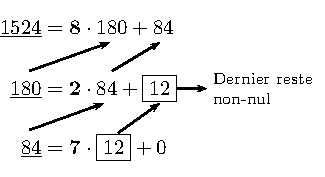
\includegraphics[scale=1]{Chapitre_2_arithmetique/figures/Correction/fig_co_1/fig_co_1.pdf}
\end{minipage}


On obtient $a=1524$ et $b=180$.




%14
\item
\begin{enumerate}[label=\alph*),itemsep=4mm]
\item 
Calculons $\pgdc(9945;3003)$ :

\hspace{6cm}\begin{minipage}[t][][b]{0.5\textwidth}
\vspace{-11.5mm}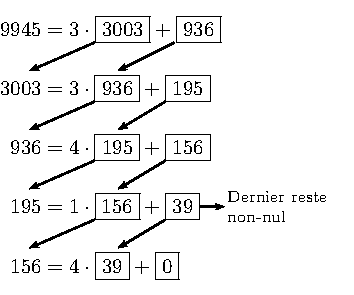
\includegraphics[scale=1]{Chapitre_2_arithmetique/figures/Correction/fig_co_2/fig_co_2.pdf}
\end{minipage}

\smallskip
Donc $\pgdc(9945;3003)=39$
\item 
$\pgdc(18480;9828)=84$
\item Par propriété du $\text{pgcd}$, pour tout entier $a$, $\text{pgcd}(-a; b) = \text{pgcd}(a; b)$.  

On a donc $\text{pgcd}(-286; 390) = \text{pgcd}(286; 390)$.

On effectue les divisions euclidiennes successives :
\begin{align*}
	390 &= 286 \cdot 1 + 104 \\
	286 &= 104 \cdot 2 + 78 \\
	104 &= 78 \cdot 1 + 26 \\
	78 &= 26 \cdot 3 + 0
\end{align*}

Le dernier reste non nul est $26$.  
Ainsi, $\text{pgcd}(-286; 390) = 26$.
\end{enumerate}


%EXERCICE
\item
\begin{itemize}\item[1)] Non car $\operatorname{PGCD}(4847 ; 5633)=131$
	
	$$
	\begin{aligned}
		5633 & =4847 \cdot 1+786 \\
		4847 & =786 \cdot 6+131 \\
		786 & =131 \cdot 6
	\end{aligned}
	$$
	
	\item[2)] Oui car $\operatorname{PGCD}(5617 ; 813)=1$
	
	$$
	\begin{aligned}
		5617 & =813 \cdot 6+739 \\
		813 & =739 \cdot 1+74 \\
		739 & =74 \cdot 9+73 \\
		74 & =73 \cdot 1+1
	\end{aligned}
	$$
\end{itemize}


%EXERCICE
\item $324=12 \cdot 27=12 \cdot 3^3$
$n$ doit être un multiple de 12 , mais pas un multiple de 36 sinon le $\operatorname{PGCD}(n ; 324)$ serait supérieur ou égal à 36 . Les entiers $n$ appartiennent à l'ensemble :
$\{12 ; 24 ; 48 ; 60 ; 84 ; 96 ; 120 ; 132 ; 156 ; 168 ; 192\}$.


%EXERCICE
\item On cherche le diviseur $b>9$ tel que :

$$
\left\{\begin{array} { l } 
	{ 1 8 0 9 = b q + 9 } \\
	{ 2 5 2 7 = b q ^ { \prime } + 7 }
\end{array} \Leftrightarrow \left\{\begin{array}{l}
	1800=b q \\
	2520=b q^{\prime}
\end{array} \Leftrightarrow\right.\right.
$$

$b>9$ et divise $\operatorname{PGCD}(4284 ; 3510)=360$
Le plus grand diviseur $b$ possible est donc 360 .



%15
\item\label{exer:pgdc_et_produit}
On note $(a;b)$ les couples de nombre entier de pgcd 14 et tels que $ab=7056$. Alors :
\begin{center}
$\left.\begin{tabular}{r}
$a=14\cdot a'$\\
$b=14\cdot b'$
\end{tabular}\right\rbrace$ avec $a'$ et $b'$ premiers entre eux.\end{center}
Comme $a\cdot b=7056$ alors $a'\cdot b'=\frac{7056}{14\cdot 14}=36$.

\medskip
Les possibilités pour $a'$ et $b'$ sont donc:
$$\boxed{\pt{1}{36}} \pvirg{4} \xcancel{\pt{2}{18}} \pvirg{4} \xcancel{\pt{3}{12}} \pvirg{4} \boxed{\pt{4}{9}} \pvirg{4} \xcancel{\pt{6}{6}}$$

Les couples qui ne sont pas premiers entre-eux ont étés barrés. Il reste donc 2 possibilités :
\renewcommand{\arraystretch}{1.4}
$$\begin{array}{r c l}
\pt{1}{36}& \overset{\cdot 14}{\longrightarrow} & \pt{14}{504} \\
\pt{4}{9} & \overset{\cdot 14}{\longrightarrow}  & \pt{56}{126}
\end{array}$$
Il y a alors deux couples vérifiant les conditions : $\pt{14}{504}$ et $\pt{56}{126}$.



%16
\item 
\begin{multicols}{2}
	\begin{enumerate}[label=\roman*),itemsep=5mm,left=-1mm,labelsep*=2mm]
		\item $3412=4\cdot 853+0$\\
		Donc $3412\equiv 0 \pmod{4}$
		\item $177=9\cdot 19+6$\\
		Donc $177\equiv 6 \pmod{9}$
		\item $31=31\cdot 1+0$\\
		Donc $31\equiv 0 \pmod{31}$
		\item $31=25\cdot 1+6$\\
		Donc $31\equiv 6 \pmod{25}$
		\item $365=5\cdot 73+0$\\
		Donc $365\equiv 0 \pmod{5}$
		\item $-3122=3\cdot (-1041)+1$\\
		Donc $-3122\equiv 1 \pmod{3}$
		\item $\nombre{31458687312}=10\cdot 3145868731+2$\\
		Donc $\nombre{31458687312}\equiv 2 \pmod{10}$
		\item $\nombre{-259874629}=10\cdot (-25987463)+1$\\
		Donc $\nombre{-259874629}\equiv 1 \pmod{10}$
	\end{enumerate}
\end{multicols}

%17
\item 
\begin{enumerate}[label=\roman*),itemsep=5mm,left=-1mm,labelsep*=2mm]
	\item[\textbf{a)}] \textbf{Vrai.} \\
	\textit{Justification :} $471 - 11 = 460$. Or $460 = 23 \cdot 20$, ce qui signifie que $23 \mid (471 - 11)$.
	
	\item[\textbf{b)}] \textbf{Faux.} \\
	\textit{Justification :} $370 - 17 = 353$. Or $353 = 13 \cdot 27 + 2$, donc $13 \nmid (370 - 17)$. \\
	(\textit{Autre méthode :} $370 = 13 \cdot 28 + 6 \implies 370 \equiv 6 \pmod {13}$ et $17 = 13 \cdot 1 + 4 \implies 17 \equiv 4 \pmod {13}$. Comme $6 \neq 4$, l'affirmation est fausse).
	
	\item[\textbf{c)}] \textbf{Vrai.} \\
	\textit{Justification :} $29 - (-121) = 29 + 121 = 150$. Or $150 = 5 \cdot 30$, donc $5 \mid (29 - (-121))$.
	
	\item[\textbf{d)}] \textbf{Faux.} \\
	\textit{Justification :} $-30 - (-1) = -30 + 1 = -29$. Or $-29$ n'est pas un multiple de $26$.
	
	\item[\textbf{e)}] \textbf{Vrai.} \\
	\textit{Justification :} Par définition de la congruence :
	\begin{itemize}
		\item $914 - 21 = 19 \cdot 47$, donc $19 \mid (914 - 21)$, d'où $914 \equiv 21 \pmod {19}$.
		\item De même, $47 \mid (914 - 21)$, d'où $914 \equiv 21 \pmod {47}$.
	\end{itemize}
	\textit{Remarque :} Bien que $21 \ge 19$ (ce n'est donc pas le reste de la division euclidienne par 19), l'égalité de congruence reste tout à fait exacte.
	
	\item[\textbf{f)}] \textbf{Vrai.} \\
	\textit{Justification :} Par définition, $b \equiv 0 \pmod a \iff b - 0 = k \cdot a \iff b = k \cdot a \iff a \mid b$.
	
	\item[\textbf{g)}] \textbf{Vrai.} \\
	\textit{Justification :} Si $b \equiv 0 \pmod a$ et $c \equiv 0 \pmod a$, alors $a \mid b$ et $a \mid c$. Par propriété de la divisibilité, $a$ divise toute combinaison linéaire $\alpha b + \beta c$ pour tous entiers $\alpha, \beta$, d'où $\alpha b + \beta c \equiv 0 \pmod a$.
\end{enumerate}

\item

\begin{itemize}
	\item \textbf{Étude de $351$ :}
	$$351 = 7 \cdot 50 + 1 \implies 351 \equiv 1 \pmod 7$$
	Par compatibilité avec les puissances :
	$$351^{12} \equiv 1^{12} \equiv 1 \pmod 7$$
	
	\item \textbf{Étude de $85$ :}
	$$85 = 7 \cdot 12 + 1 \implies 85 \equiv 1 \pmod 7$$
	Par compatibilité avec les puissances :
	$$85^{15} \equiv 1^{15} \equiv 1 \pmod 7$$
	
	\item \textbf{Produit :}
	Par compatibilité avec la multiplication :
	$$351^{12} \cdot 85^{15} \equiv 1 \cdot 1 \equiv 1 \pmod 7$$
\end{itemize}



% exo
\item

\begin{enumerate}
	\item \textbf{Étude du premier terme $5^{2n}$ :}
	On réécrit la puissance à l'aide des règles de calcul :
	$$5^{2n} = \left(5^2\right)^n = 25^n$$
	
	Or, $25 = 11 \cdot 2 + 3$, donc :
	$$25 \equiv 3 \pmod{11}$$
	
	Par compatibilité de la congruence avec les puissances, on a :
	$$5^{2n} \equiv 3^n \pmod{11}$$
	
	\item \textbf{Étude du second terme $14^n$ :}
	On effectue la division euclidienne de $14$ par $11$ :
	$$14 = 11 \cdot 1 + 3 \implies 14 \equiv 3 \pmod{11}$$
	
	Par compatibilité de la congruence avec les puissances, on a :
	$$14^n \equiv 3^n \pmod{11}$$
	
	\item \textbf{Soustraction des congruences :}
	Par compatibilité avec la soustraction :
	$$5^{2n} - 14^n \equiv 3^n - 3^n \pmod{11}$$
	$$5^{2n} - 14^n \equiv 0 \pmod{11}$$
\end{enumerate}

\textbf{Conclusion :} 
Pour tout entier naturel $n$, $5^{2n} - 14^n$ est divisible par $11$.


%17
\item
\begin{enumerate}[label=\roman*),itemsep=5mm,left=-1mm,labelsep*=2mm]
	\item $\phantom{195}1=13\cdot 0+1$\\
	$1951=13\cdot 150+1$\\
	$1964=13\cdot 151+1$\\
	$1977=13\cdot 152+1$\\
	$1990=13\cdot 153+1$ \eh{4} Donc, $1\equiv 1951 \equiv 1964 \equiv 1977 \equiv 1990 \pmod{13}$
	
	\item $1776=40\cdot 44+16$\\
	$1976=40\cdot 49+16$ \eh{4} Donc, $16\equiv 1776 \equiv 1976  \pmod{40}$
	
	\item $1929=15\cdot 128+9$\\
	$1959=15\cdot 130+9$\\
	$1974=15\cdot 131+9$\\
	$1989=15\cdot 132+9$ \eh{4} Donc, $9\equiv 1929 \equiv 1959 \equiv 1974 \equiv 1989 \pmod{15}$
	
\end{enumerate}




%18
\item 
\begin{enumerate}[label=\arabic*),itemsep=3mm,left=-1mm,labelsep*=2mm]
	\item On vérifie la véracité de la proposition pour $n=0$ et $n=1$ :
	
	\smallskip
	$6\cdot 4^0=6=9\cdot 0 +6$ donc $6\cdot 4^0\equiv 6 \pmod{9}$
	
	\smallskip
	$6\cdot 4^1=24=9\cdot 2 +6$ donc $6\cdot 4^1\equiv 6 \pmod{9}$
	
	\item Supposons que $6\cdot 4^n\equiv 6 \pmod{9}$ pour un certain $n\in \N$ et montrons que la proposition est vraie pour $n+1$.
	
	\smallskip
	Comme $6\cdot 4^n\equiv 6 \pmod{9}$, par définition cela signifie que $\exists k\in \Z$ tel que $6\cdot 4^n=6+9k$. On a alors :
	$$6\cdot 4^{n+1}=6\cdot 4^n\cdot 4=(6+9k)\cdot 4=24+36k=6+18+36k=6+9(2+4k)$$
	
	On pose $k'=2+4k$ et on obtient $6\cdot 4^{n+1}=6+9k'$.
	
	\smallskip
	On conclut alors que $6\cdot 4^{n+1} \equiv 6 \pmod{9}$
\end{enumerate}
\clearpage



%19
\item
Il s'agit de calculer $100^{1000}$ modulo $13$. 

\smallskip
Tout d'abord remarquons que $100 \equiv 9 \pmod{13}$ donc  $100^{1000} \equiv 9^{1000} \pmod{13}$. 

\smallskip
Puis, plusieurs raisonnements sont possibles. En voici deux :

\begin{enumerate}[label=\roman*)]
	\item $9^{2} \equiv 81 \equiv 3 \pmod{13}$ et donc $9^{3} \equiv 9^2\cdot 9 \equiv 3\cdot 9 \equiv 1 \pmod{13}$
	
	On conclut avec: $$100^{1000} \equiv 9^{1000} \equiv 9^{3\cdot 333+1} \equiv \left(9^3\right)^{333}\cdot9  \equiv 1^{333}\cdot9 \equiv 9 \pmod{13}$$
	
	\item $9^{2} \equiv 81 \equiv 3 \pmod{13}$ et donc $9^{5} \equiv \left(9^2\right)^2\cdot 9 \equiv 3^2\cdot 9 \equiv 81 \equiv 3 \pmod{13}$.
	
	On déduit que $9^{10} \equiv \left(9^5\right)^2 \equiv 3^2 \equiv  9 \pmod{13}$
	
	On conclut avec : $$100^{1000} \equiv 9^{1000} \equiv \left(\left(9^{10}\right)^{10}\right)^{10} \equiv \left(9^{10}\right)^{10}  \equiv 9^{10} \equiv 9 \pmod{13}$$
\end{enumerate}




%20
\item
Raisonnons modulo $8$ et remarquons que $7 \equiv -1 \pmod{8}.$

\smallskip
D'où on tire :
$$7^n +1 \equiv (-1)^n + 1 \pmod{8}.$$

Le reste de la division euclidienne de $7^n+1$ par $8$ est $r(n)=(-1)^n+1$.

\begin{itemize}
	\item Si $n$ est impair alors $r(n)=(-1)^n+1=0$ et $7^n+1$ est divisible par $8$.
	
	\item Si $n$ est pair alors $r(n)=(-1)^n+1=2$ et $7^n+1$ n'est pas divisible par $8$ (et le reste vaut $2$).
\end{itemize}




%21
\item
\begin{enumerate}[label=\alph*),itemsep=5mm,left=-1mm,labelsep*=2mm]
	\item $12 \equiv 1 \pmod{11} \Rightarrow 12^{15} \equiv 1 \pmod{11}$.
	
	\ev
	Le reste de la division de $12^{15}$ par 11 est 1.
	\item $10 \equiv -1 \pmod{11} \Rightarrow 10^{7} \equiv -1 \equiv 10 \pmod{11}$.
	
	\ev
	Le reste de la division de $10^{7}$ par 11 est 10.
	\item $78 \equiv 1 \pmod{11} \Rightarrow 78^{15} \equiv 1 \pmod{11}$.
	
	\ev
	Le reste de la division de $78^{15}$ par 11 est 1.
	\item $13 \equiv 2 \pmod{11} \Rightarrow 13^{12} \equiv 2^{12} \pmod{11}$.
	
	\ev
	Nous avons $2^4=16 \equiv 5 \pmod{11} \Rightarrow \left(2^4\right)^3 \equiv 125 \equiv 4 \pmod{11}$.
	
	\ev
	Le reste de la division de $13^{12}$ par 11 est 4.
	\item $\left(-2\right)^6 = 64 \equiv -2 \pmod{11}$.
	
	\ev
	Nous avons $\left(-2\right)^{19} = \left(\left(-2\right)^6\right)^3\cdot(-2) \equiv \left(-2\right)^3\cdot(-2) \equiv 16 \equiv 5 \pmod{11}$.
	
	\ev
	Le reste de la division de $\left(-2\right)^{19}$ par 11 est 5.
\end{enumerate}




%22
\item
\begin{enumerate}[label=\alph*),itemsep=5mm,left=-1mm,labelsep*=2mm]
	\item \begin{itemize}\setlength{\itemsep}{2mm}
		\item $2^4=17\cdot 1 -1  \eh{1}\Rightarrow\eh{1} 2^4\equiv -1 \pmod{17}$.
		\item $6^2=17\cdot 2 +2  \eh{1}\Rightarrow\eh{1} 6^2\equiv 2 \pmod{17}$.
	\end{itemize}
	
	\item \begin{itemize}\setlength{\itemsep}{2mm}
		\item On a $1532=90\cdot 17 +2$. Donc $[1532]_{17}=[2]_{17}$
		\item On a $346=20\cdot 17 +6$. Donc : $[346]_{17}=[6]_{17}$ 
	\end{itemize}
	
	\item \begin{itemize}\setlength{\itemsep}{2mm}
		\item $1532^{20}\equiv 2^{20} \equiv\left(2^4\right)^5 \equiv (-1)^5 \equiv -1 \equiv 16 \pmod{17}.$
		
		\smallskip
		Le reste de la division de $1532^{20}$ par 17 est 16.
		\item $346^{12}\equiv 6^{12} \equiv\left(6^2\right)^6 \equiv 2^6 \equiv 2^4\cdot 4 \equiv -4 \equiv 13 \pmod{17}.$
		
		\smallskip
		Le reste de la division de $346^{12}$ par 17 est 13.
	\end{itemize}
\end{enumerate}




%23
\item
\begin{multicols}{3}
	\begin{enumerate}[label=\alph*)]
		\item $S= \lbrace \left[6\right]_7\rbrace$
		\item $S= \lbrace \left[11\right]_{30} \; ; \; \left[26\right]_{30} \rbrace$
		\item[]
	\end{enumerate}
\end{multicols}




%24
\item
\begin{enumerate}[label=\alph*),itemsep=7mm,left=-1mm,labelsep*=2mm]
	\item\label{a} Soit $n$ un nombre impair, alors il s'écrit $n=2k+1$ avec $k\in \Z$. Alors :
	
	$$n^2 = (2k+1)^2 = 4k^2+4k+1 = 4k(k+1) + 1.$$ Par ailleurs, de $k$ ou $k+1$ l'un des deux est pair, donc $4k(k+1)$ est un multiple de 8.
	
	Donc $n^2 \equiv 1 \pmod{8}$ et le reste de la division de $n^2$ par $8$ est $1$.
	
	\item\label{b} Si $n$ est pair alors il existe $k\in \Z$ tel que $n=2k$ et $n^2 = 4k^2$.
	
	\begin{itemize}
		\item Si $k$ est pair alors il existe $j\in \Z$ tel que $k=2j$ et $k^2=4j^2$.
		
		Donc $n^2 = 4k^2 = 16j^2$ est divisible par $8$. Finalement $n^2 \equiv 0 \pmod{8}$.
		
		\item Si $k$ est impair alors il existe $j\in \Z$ tel que $k=2j+1$ et $k^2=4j^2+4j+1$.
		
		Donc $n^2 = 4k^2=16(j^2+j)+4$ est divisible par 4 mais pas par 8.
		
		Finalement $n^2 \equiv 4 \pmod{8}$. 
	\end{itemize}
	
	\item\label{c} \begin{itemize}\setlength{\itemsep}{4mm}
		\item Comme $a, b, c$ sont impairs alors d'après la question \ref{a} on a :
		
		\medskip
		\centerline{$a^2 \equiv 1 \pmod{8}$\ehh,\ehh $b^2 \equiv 1 \pmod{8}$\ehh,\ehh$c^2 \equiv 1 \pmod{8}$.}
		
		\medskip
		Donc $a^2+b^2+c^2 \equiv 1+1+1 \equiv 3 \pmod{8}$.
		
		\item On écrit $a = 2k+1$, $b=2j+1$ et $c=2i+1$, alors :
		$$2ab = 2(2k+1)(2j+1) = 8kj + 4(k+j)+2$$
		$$2bc = 2(2j+1)(2i+1) = 8ji + 4(j+i)+2$$
		$$2ac = 2(2k+1)(2i+1) = 8ki + 4(k+i)+2$$
		Donc :
		$$2(ab+bc+ca)= 8kj+8ji+8ki + 8(k+j+i)+6= 8(kj+ji+ki+k+j+i)+6$$
		Finalement $2(ab+bc+ca) \equiv 6 \pmod{8}$.
	\end{itemize}
	
	\item \begin{enumerate}[label=\roman*)] 
		\item Montrons par l'absurde que le nombre $a^2+b^2+c^2$ n'est pas le carré d'un nombre entier.
		
		\smallskip
		Supposons qu'il existe $n\in \N$ tel que $a^2+b^2+c^2=n^2$. 
		
		\smallskip
		D'une part, nous avons montré au point \ref{c} que $a^2+b^2+c^2 \equiv 3 \pmod{8}$.
		
		\smallskip
		D'autre part, nous avons montré au point \ref{b} que si $n$ est impair alors $n^2 \equiv 1 \pmod{8}$ et si $n$ est pair alors
		$n^2 \equiv 0 \pmod{8}$ ou $n^2 \equiv 4 \pmod{8}$.
		
		\smallskip
		Dans tous les cas $n^2$ n'est pas congru à $3$ modulo $8$. Donc il y a une contradiction et nous concluons que $a^2+b^2+c^2$ n'est pas un carré.
		
		\item On fait le même raisonnement avec $2(ab+bc+ca)$.
		
		\item Pour $ab+bc+ca$ l'argument est similaire : 
		d'une part $2(ab+bc+ca)\equiv 6 \pmod{8}$
		et d'autre part si, par l'absurde, on suppose $ab+bc+ca=n^2$ alors
		selon la parit\'e de $n$ nous avons $2(ab+bc+ca)\equiv 2n^2 \equiv 2 \pmod{8}$
		ou \`a $0 \pmod{8}$. Dans les deux cas cela aboutit à une contradiction. On conclut que
		$ab+bc+ca$ n'est pas un carré.
	\end{enumerate}
\end{enumerate}




%16
\item
\begin{enumerate}[label=\alph*),itemsep=4mm]
\item
En effectuant la remontée de l'algorithme d'Euclide on obtient:
$$\pgdc(7260;637)=1=\bm{(141)}\cdot 7260 + \bm{(-1607)}\cdot 637$$
\item
En effectuant la remontée de l'algorithme d'Euclide on obtient:
$$\pgdc(9945;3003)=39=\bm{(-16)}\cdot 9945 + \bm{(53)}\cdot 3003$$
\end{enumerate}





%17
\item
On utilise le corolaire 2.6 et on pose $u=-1$ et $v=1$ : $(-1)\fois a+1\fois(a+1)=1$. Donc $\pgdc(a;a+1)=1$.




\clearpage
%18
\item
\begin{enumerate}[label=\alph*),itemsep=1mm]
\item $x=241 \et{2} y=-364$. \eh{2} On obtient $873\fois \bm{241}+578\fois \bm{(-364)}=1$
\item $x=-345 \et{2} y=190$ \eh{2} On obtient $315\fois \bm{(-345)}+572\fois \bm{(190)}=5$
\item Cette équation n'a pas de solution dans $\Z^2$. {\small(La somme ou la différence de deux nombres paires sera toujours paire)}
\end{enumerate}




%19
\item
Il faut utiliser le fait que\eh{1} $\pgdc(a;b)\fois \ppmc(a;b)=\vert ab\vert$. On déduit que $\vert ab\vert=5184$.

\smallskip
On fait le même raisonnement qu'à l'exercice \ref*{exer:pgdc_et_produit} et on trouve: $\pt{\pm 12}{\pm 432}$ et $\pt{\pm 48}{\pm 108}$ {\small (soit $8$ couples)}. 



%20
\item



%21
\item




%22
\item \begin{minipage}[t][][b]{1\textwidth}
\insertcode{Chapitre_2_arithmetique/Programmes/Eratosthene.py}{0.9}{}
\end{minipage}




%23
\item
Par exemple $5x-2y=-24$.

\smallskip
Il suffit de choisir aléatoirement $a,b \in \N$ puis de calculer $c\in \N$ tel que $a\cdot 24+b\cdot 72=c$.




%24
\item
\begin{enumerate}[label=\alph*),itemsep=5mm,left=-1mm,labelsep*=2mm]
\vspace{-3mm}
\item Il faut résoudre le système d'équations suivant dans $\Z$:
$\left\lbrace\begin{array}{@{\eh{1}}r@{\eh{1}}c@{\eh{1}}c@{\eh{1}}c@{\eh{1}}l}
6a   & + & 17b & = & c\\
-18a & - & 23b & = & c\\
\end{array}\right.$

S'agissant d'un système sous-déterminé, il possède une infinité de solutions toutes de la forme :
$$\left(-\frac{5}{21}\alpha\; ;\; \frac{1}{7}\alpha \; ;\; \alpha \right)$$

Pour que les solutions soient entières, il faut que $\alpha$ soit un multiple de ppmc$(7,21)=21$. 

\smallskip
Finalement nous obtenons : $S=\lbrace \left(-5\beta\; ;\; 3\beta \; ;\; 21\beta \right) \mid \beta\in \Z \rbrace$

\smallskip
On conclut que toute équation de la forme $-5\beta\cdot x+ 3\beta\cdot y = 21\beta$ avec $\beta\in \Z$ est une équation diophantienne ayant $(6;17)$ et $(-18;-23)$ pour solutions.

\item Comme nous venons de le voir, il existe une infinité d'équations ayant pour solutions $(6;17)$ et $(-18;-23)$, cependant ces équations sont toutes équivalentes. On peut remarquer que les solutions d'une équation du type $ax+by=c$ forment une droite. Par deux points passant une et une seule droite (1er axiome d'Euclide), l'équation cherchée est donc celle d'une droite, qui peut être donnée par une infinité d'équations mais toutes équivalentes. 
\end{enumerate}




%25
\item 
Grâce à l'algorithme d'Euclide nous trouvons que pgcd$(1665;1035)=45$. Comme $45\ | \ 45$, la proposition 2.14 assure que cette équation possède des solutions. La remontée de l'algorithme fourni une solution particulière à l'équation (les coefficients de Bézout) : 
$$1665\cdot \bm{5} + 1035 \cdot \bm{(-8)} = 45$$
Une solution particulière de $(E)$ est donc $(x_0,y_0) = (5,-8)$.

%\medskip
%Nous allons maintenant trouver l'expression générale pour les solutions de l'équation $(E)$.

\medskip
Soit alors $(x,y)$ une solution quelconque de l'équation $1665x+1035y=45$. Comme $(x_0,y_0)$ est aussi solution, nous avons $1665x_0+1035y_0=45$. En faisant la différence de ces deux égalités nous obtenons :

$$1665(x-x_0)+1035(y-y_0)=0 \quad\ssi$$
$$1665(x-x_0)=-1035(y-y_0) \quad\overset{:45}{\ssi}$$
$$37(x-x_0)=-23(y-y_0) \quad (*)$$

\medskip
On en déduit que $37\ |\ -23 (y-y_0)$ et comme pgcd$(37;23)=1$ le lemme de Gauss assure que
$37\ |\ (y -y_0)$ (c'est ici qu'il est important d'avoir divisé par $45$!).

\medskip
Cela nous permet d'écrire $y-y_0 = 37 k$ pour un $k \in \Z$. Repartant de l'égalité $(*)$ nous obtenons alors  : $37(x-x_0)=-23 \cdot 37 \cdot k$.
Ce qui donne $x-x_0 = -23 k$.

\medskip
Donc si $(x,y)$ est solution de $(E)$ alors elle est de la forme :
$(x,y)= (x_0 - 23k,y_0+37k)$, avec $k \in \Z$.

Réciproquement pour chaque  $k\in\Z$, si $(x,y)$ est de cette forme alors c'est une solution de $(E)$
(vérifiez-le !).\\
Finalement  :
$$S=\big\lbrace (5 - 23k,-8+37k) \mid k\in \Z\big\rbrace.$$



%26
\item
L'algorithme d'Euclide donne pgcd$(35;84)=7$.
%\begin{align*}
%84 & =35\cdot 2 +14\\
%35 & = 14\cdot 2 +7\\
%14 & =7\cdot 2 +0
%\end{align*}

\medskip
Attendu que $7$ ne divise pas $150$, l'équation diophantienne $35x+84y=150$ n'admet pas de solution entière. La droite d'équation $35x+84y=150$ ne passe donc par aucun point à coordonnées entières et ne croise donc jamais une intersection du quadrillage.
%pour déterminer le pgcd de $35$ et $84$ donne :




%27
\item
\begin{enumerate}[label=\alph*),itemsep=5mm,left=-1mm,labelsep*=2mm]
\item Soit : \begin{minipage}[t]{0.9\textwidth}
$\boldsymbol{x} :$ le nombre d'étudiants ayant participé au repas.

\smallskip
$\boldsymbol{y} :$ le nombre d'enfants ayant participé au repas.

\smallskip
$\boldsymbol{28-x-y} :$ le nombre d'adultes ayant participé au repas.
\end{minipage}

\smallskip
Le problème se traduit donc par l'équation diophantienne :\vspace{-1mm}
$$17x+13y+26(28-x-y)=613 \ehhh \ssi \ehhh \boldsymbol{9x+13y=115} \ehh \textrm{(E)}$$

\item Le couple $(3\; ;-2)$ est une solution évidente de $9x+13y=1$, donc :
$$\left(115\cdot 3\; ; 115\cdot (-2)\right)=(345\;-230)$$ est une solution particulière de (E).
En soustrayant la solution particulière de la solution générale, on trouve :
$$9(x-345)=13(-230-y)$$
Comme pgcd$(13\; ; 9)=1$, on en déduit, d'après le lemme de Gauss, que $13$ divise $x-345$ et que $9$ divise $(-230-y)$. On trouve alors :
\renewcommand{\arraystretch}{1.3}
$$\left\lbrace\begin{array}{l}
x=13k+345\\
y=-9k-230
\end{array}\right. \textrm{avec } k\in \Z$$
Comme $x$ et $y$ sont des nombres positifs, on a :
$$\left\lbrace\begin{array}{l}
13k+345\geqslant 0\\
-9k-230 \geqslant 0
\end{array}\right. \ehhh \ssi \ehhh \renewcommand{\arraystretch}{2.2}%%%%%%%%%%%%%%%%%%%
\left\lbrace\begin{array}{l}
k\geqslant -\frac{345}{13}\simeq -26,5\\
k \leqslant -\frac{230}{9}\simeq -25,6
\end{array}\right.$$
La seule valeur possible est alors $k=-26$ et on trouve $x=7$ et $y=4$.

\smallskip
Il y a donc 7 étudiants, 4 enfants et 17 adultes.
\item  ~

\vspace{-5mm}
\begin{center}
\comp{\fbox{\begin{minipage}[t]{0.72\textwidth}\setlength{\arrayrulewidth}{2pt}

\textbf{Variable :} $x$, $y$ (entiers)\\
\textbf{Début}

\vspace{2mm}
\begin{tabular}{|c}
\begin{minipage}{\textwidth}
	\textbf{Pour} $x$ de 0 à 28 \textbf{Faire}\vspace{2mm}\\
	\begin{tabular}{|c}
	\begin{minipage}{\textwidth}
			\textbf{Pour} $y$ de 0 à 28 \textbf{Faire}\vspace{2mm}\\
			\begin{tabular}{|c}\vspace{2mm}
			\begin{minipage}{\textwidth}
					\textbf{Si} $9x+13y=115$ \textbf{Alors}\\
					\begin{tabular}{|c}
					\begin{minipage}{\textwidth}
						\textbf{Afficher} "Il y a " x " étudiants et " y " enfants."
					\end{minipage}
					\end{tabular}\vspace{1mm}\\
					\textbf{FinSi}
			\end{minipage}
			\end{tabular}\vspace{1mm}\\
			\textbf{FinPour}
	\end{minipage}
	\end{tabular}\vspace{3mm}\\
	\textbf{FinPour}
\end{minipage}
\end{tabular}

\vspace{2mm}
{\bf Fin}
\end{minipage}}}
\end{center}
\end{enumerate}












\end{enumerate}





















\clearpage
 ~
\newpage
%
%
%
%%\chapter{Continuité et Asymptotes}
%\renewcommand{\titrechapitre}{Continuité et Asymptotes}
%\thispagestyle{fancy}
%\input{Chapitre_2_continuite_asymptotes/2.Continuite_Asymptotes-CORRECTION}
%\clearpage
%
%
%%\setcounter{page}{21}
%%\setcounter{chapter}{3}
%%\chapter{Calcul Différentiel}
%\renewcommand{\titrechapitre}{Calcul Différentiel}
%\thispagestyle{fancy}
%\input{Chapitre_3_derivees/3a.Derivees-CORRECTION}
%\clearpage



%\colorlet{couleurchapitre}{orange!75!black}
%\setcounter{page}{1}
%\setcounter{chapter}{4}
%\renewcommand{\titrechapitre}{Géométrie Vectorielle \& Analytique}
%\thispagestyle{fancy}
%\columnsep=40pt
%\raggedcolumns
%\begin{multicols*}{2}
%\raggedcolumns
%\columnseprule=1.pt
%\renewcommand{\columnseprulecolor}{\color{gray}}
%\input{Chapitre_4_geometrie_vectorielle-analytique/4a.Vecteurs-CORRECTION}
%\end{multicols*}
%\clearpage




%\colorlet{couleurchapitre}{orange!75!black}
%\setcounter{page}{1}
%\setcounter{chapter}{5}
%\renewcommand{\titrechapitre}{Géométrie Analytique}
%\thispagestyle{fancy}
%\columnsep=40pt
%\raggedcolumns
%\begin{multicols*}{2}
%\raggedcolumns
%\columnseprule=1.pt
%\renewcommand{\columnseprulecolor}{\color{gray}}
%\input{Chapitre_5_geometrie_analytique/5a.Droites-CORRECTION}
%\end{multicols*}
%\clearpage




\end{document}














